%\documentclass[aip,pop,amsmath,amssymb,preprint]{revtex4-1} %preprint version
\documentclass[aip,pop,amsmath,amssymb,reprint,superscriptaddress]{revtex4-1} %preprint version
\usepackage{graphicx}% Include figure files
\usepackage{dcolumn}% Align table columns on decimal point
\usepackage{bm}% bold math

    \renewcommand{\topfraction}{0.9}    % max fraction of floats at top
    \renewcommand{\bottomfraction}{0.8}    % max fraction of floats at bottom
    \setcounter{topnumber}{2}
    \setcounter{bottomnumber}{2}
    \setcounter{totalnumber}{4}     % 2 may work better
    \setcounter{dbltopnumber}{2}    % for 2-column pages
    \renewcommand{\dbltopfraction}{0.9}    % fit big float above 2-col. text
    \renewcommand{\textfraction}{0.07}    % allow minimal text w. figs
    \renewcommand{\floatpagefraction}{0.7}    % require fuller float pages
    \renewcommand{\dblfloatpagefraction}{0.7}    % require fuller float pages
    \setlength{\abovecaptionskip}{5pt}
    \setlength{\belowcaptionskip}{5pt}
    \setlength{\parskip}{0pt}
    \setlength{\textfloatsep}{5pt} 

\begin{document}
\title{Turbulence and Transport Suppression Scaling with Bias-driven Variation of Flow Shear on the Large Plasma Device}
\author{D.A. Schaffner}
\author{T.A Carter}
\author{G.D. Rossi}
\author{D.S. Guice}
\author{J.E. Maggs}
\author{S. Vincena}
\author{B. Friedman}
\affiliation{Department of Physics and Astronomy, University of California, Los Angeles}
\date{\today}
\begin{abstract}
Continuous control over azimuthal flow and shear in the edge of the Large Plasma Device (LAPD) has been achieved using a biasable limiter which has allowed a careful study of the effect of flow shear on pressure-gradient-driven turbulence and transport in LAPD. The combination of such fine shear variation in a fully turbulent plasma along with the detailed spatial diagnostic capabilities on LAPD makes the experiment a useful testbed for verification and comparison to various shear suppression models. Power-law fits are made to the density and radial velocity fluctuation amplitude, particle flux, relative crossphase between density and velocity fluctuations and radial correlation length as functions of both weak and strong shearing. Model comparisons with experimental results are mixed; some models make favorable predictions for certain quantities but not others. Overall, the combination of scattered predictions and experimental results suggest that shear suppression may be turbulence-type dependent.
\end{abstract}
\maketitle

\section{Introduction}

Suppression of turbulence and transport by increased flow shear has been observed on a multitude of different plasma experiments in both spontaneous flow states as well as bias driven flow~\cite{burrell99,oost03,sakai93}. While the necessity of cross-field flow shear has been generally accepted for the successful high confinement operation of current and future plasma devices, the exact physical mechanisms connecting increased flow shear to the suppression of turbulence and transport is not fully understood. Having a quantitative grasp as to how turbulence and confinement levels scale with flow shear as well as the ability to make predictions as to what mechanisms will dominate in various scenarios is vital for extrapolation to larger future machines such as ITER~\cite{burrell97,terry00}. The primary goal of this paper is to provide a detailed experimental dataset for comparison and verification of various models which make predictions as to the relative magnitude of suppression for various turbulent quantities. A further goal is to provide insight into the physical mechanisms actually at work in such suppression observations.

Control of polodial or azimuthal flow shear in a turbulent plasma has been previously achieved in a number of torodial devices using biased electrodes in order to create cross-field flow through the generation of cross-field current~\cite{taylor89,weynants92}. In particular, biasing experiments conducted on TEXTOR~\cite{weynants98,boedo00,boedo02} have yielded results that have been compared to shear suppression models for both density fluctuation amplitude and particle flux showing promising comparisons. Using a recent dataset on LAPD~\cite{schaffner12} where a detailed scan of sheared flow in a turbulent, linear field line plasma was made using a biased limiter, we hope to extend such shear suppression model verification studies. The recent data set demonstrated the suppression and modification of a number of turbulent quantities with increased shearing rate including cross-field particle flux, density and radial $E\times B$ velocity fluctuations, the relative crossphase between said fluctuations, and radial correlation length. Moreover, the scan included data points in both the weak and strong shearing regime, as defined by the ratio of shearing rate to inverse autocorrelation time providing the ability for comparison to models which make separate predictions for each regime.

\section{Suppression Modeling}

Shear suppression models based on the spatial decorrelation of turbulent structures has been the most common approach to describing both the physical mechanism underlying suppression as well as for making scaling predictions~\cite{terry00}. The basic premise underlying these models is the effect of shearing to break apart or shrink turbulent eddies and consequently decrease both fluctuation amplitude and transport step size. Variation in the model predictions arise from differences in shearing regime, source of turbulent drive (i.e. Ion Temperature Gradient, Interchange Drive or Pressure-Gradient Drive), as well as consideration of passive versus dynamic scalars. Recently, other approaches to explaining shear suppression have been made including the enhancement of coupling to damped eigenmodes by sheared flow~\cite{terry06} and by nonlinear shifts in the wavenumber spectrum of the turbulence by shearing(Staebler, APS 2012). However, this paper will focus on the varying decorrelation models which include scaling predictions. 

Two of the earliest of decorrelation models were developed by Biglari, Diamond, Terry~\cite{biglari90} and Shaing~\cite{shaing90}. The BDT theory presents a generalized analysis of the transport of any passive scalar in a mean sheared flow in the strong-shear regime with constant drive gradient. The BDT model predicts that normalized fluctuation amplitude scales directly with shear to the -2/3 power as in,
%
\begin{equation}
\frac{\langle |\tilde{\xi}|^{2} \rangle}{\langle |\tilde{\xi}|^{2} \rangle}_{\gamma_{s}=0} \sim (\gamma_{s}\tau_{ac})^{-2/3}
\label{eq:BDT_theory}
\end{equation}
%
where $\eta$ can be any quantity such as density or temperature. Conversely, the Shaing model predicts a scaling of the form,
%
\begin{equation}
\frac{\langle |\tilde{\xi}|^{2} \rangle}{\langle |\tilde{\xi}|^{2} \rangle}_{\gamma_{s}=0} \sim 1- \alpha(\gamma_{s}\tau_{ac})^2
\label{eq:shaing_theory}
\end{equation}
%
for fluctuation amplitude for the weak shear regime, where $\alpha$ is a constant containing mode number information. An attempt to incorporate the BDT and Shaing models was made by Zhang and Mahajan~\cite{zhang92,zhang93}by expanding the model to incorporate the self-consistent modification of the diffusion and spectrum through fluctuation changes by the flow shear (allowing for a distinction between weak and strong turbulence regimes in the shearing model). The resulting model shows correspondence to the Shaing model in the weak shearing regime while the BDT model is recovered in the strong shearing regime but only for the case where diffusion is unchanged by fluctuation amplitude changes. Furthermore, they extend the model to incorporate the effect of changes in gradient length, showing that shear suppression of fluctuation amplitude is enhanced by a steeper equilibrium gradient. 

Work by Ware and Terry~\cite{ware96,ware98} made predictions for the effect of shearing on particle transport specifically in a resistive pressure-gradient driven turbulence state. Their work predicted a decrease in flux as a $\Gamma_{p} \sim 1-\gamma_{s}^2$ model in the weak shear limit as well as predicting a decrease in the cosine of the crossphase between density and radial velocity fluctuations also of the form $1-\omega_{s}^2$. They, too, incorporated the modification of the pressure gradient formulating an expression for shearing suppression of radial particle diffusivity of the form,
%
\begin{equation}
\frac{D}{D(\gamma_{s}=0)} \sim 1-\beta(\gamma_{s})^2
\label{eq:ware_diff_theory}
\end{equation}
%
where $\beta$ is a constant containing the linear growth rate and radial mode width.

Further work by Terry, Newman and Ware~\cite{terry01} examined the modification of flux in the strong shearing regime for a non-mode-specific turbulence system, prediction a direct scaling of $\Gamma_{p} \sim \gamma{s}^{-4}$ overall, with fluctuation amplitude reductions contributing one power while crossphase reduction contributed three powers, suggesting both a strong dependence of flux on shear as well as an implication that the crossphase can be the dominant flux suppression mechanism rather than the fluctuation amplitude. However, Kim and Diamond~\cite{kim03}recast the decorrelation model to include resonance absorption between the shear flow and fluctuations overall suggesting a much weaker dependence of flux on shear,$\Gamma_{p} \sim \gamma_{s}^{-1}$, and even weaker dependence of crossphase, $\cos(\theta_{nv_{r}}) \sim \gamma_{s}^{-1/6}$, while fluctuations decreased as $|\tilde{n}|^{2} \sim \gamma_{s}^{-5/3}$. Additional work~\cite{kim04} added the effect of treating the fluctuating flows dynamically in an interchange driven turbulent plasma which allowed for a prediction for the decrease in fluctuating radial velocity as a function of shear scaling as $|\tilde{v_{r}}|^{2} \sim \gamma_{s}^{-3}$ in weak shear, and $|\tilde{v_{r}}|^{2} \sim \gamma_{s}^{-4}$ in strong shearing.

Most recently, Leconte et al~\cite{leconte06} found different scalings for flux, fluctuations and crossphase in the strong shear regime depending on relative shearing strength relative to a characteristic time and shearing spatial gradient relative to the inhomogeneity gradient. Work by Newton and Kim has utilized numerical simulations to determine shearing scalings in a generic model~\cite{newton07,newton11}.

\section{Bias Shearing Experiments on LAPD}

The Large Plasma Device \cite{gek91} (LAPD) is a 17m long, $\sim$60cm diameter cylindrical plasma produced by a barium-oxide coated nickel cathode. In the experiments reported here, a plasma of density $\sim$$2 \times 10^{12}$ cm$^{-3}$ and peak temperature of ~8eV is produced in a uniform solenoidal magnetic field of 1000G.  Measurements of electron density, electron temperature, and potential (both plasma potential and floating potential) are made using Langmuir probes.   Measurements of ion saturation current ($I_{\rm sat} \propto n_e \sqrt{T_e}$) and floating potential ($V_f$) are taken with a 9-tip Langmuir probe (flush-mount tantalum tips) while temperature and plasma potential are determined using a swept Langmuir probe. $I_{\rm sat}$ fluctuations are taken as a proxy for density fluctuations for the measurements reported in this work. Density profiles are determined by scaling averaged $I_{\rm sat}$ profiles to line-averaged interferometer measurements of density.  Turbulent particle flux $\Gamma \propto \left<\tilde{n}_e \tilde{E}_\theta\right>$ is determined through correlating density fluctuations from one tip of this probe with azimuthal electric field fluctuations ($E_\theta$) derived from floating potential fluctuations on two azimuthally separated tips. Azimuthal $E\times B$ flow is computed using the swept-probe-derived plasma potential. 

A large annular aluminum limiter was installed in LAPD to provide a parallel boundary condition for the edge plasma and is biased relative to the cathode of the plasma source to control plasma potential and cross-field flow.  The limiter is an iris-like design with four radially movable plates located 2.5m from the cathode as shown schematically in Fig.~\ref{fig:velocity_flowshear}(a).  The limiters create a 52cm diameter aperture; downstream of the limiter, plasma on field lines with radial location $r>26$cm has the limiter as a conducting end parallel boundary condition and plasma on field lines for $r<26$cm has the anode/cathode of the source region as a parallel boundary condition.  An electrically floating conducting end mesh terminates the plasma on the far end of the device.  A capacitor bank and transistor switch supply a voltage pulse to the limiter.  The bias pulse lasts 5ms during the flat-top of the $\sim$$15$ms plasma  discharge. The limiter is biased from $\sim$$10$V below to 50V above the anode potential.  Typically, plasma potential in the core LAPD plasma (plasma on field lines that connect to the source region) is very close to the anode voltage and the cathode sits near ground (vacuum chamber wall).  The anode potential is above the cathode potential by the discharge voltage, which was $\sim$$40$V during these experiments.

\begin{figure}[!htbp]
\centerline{
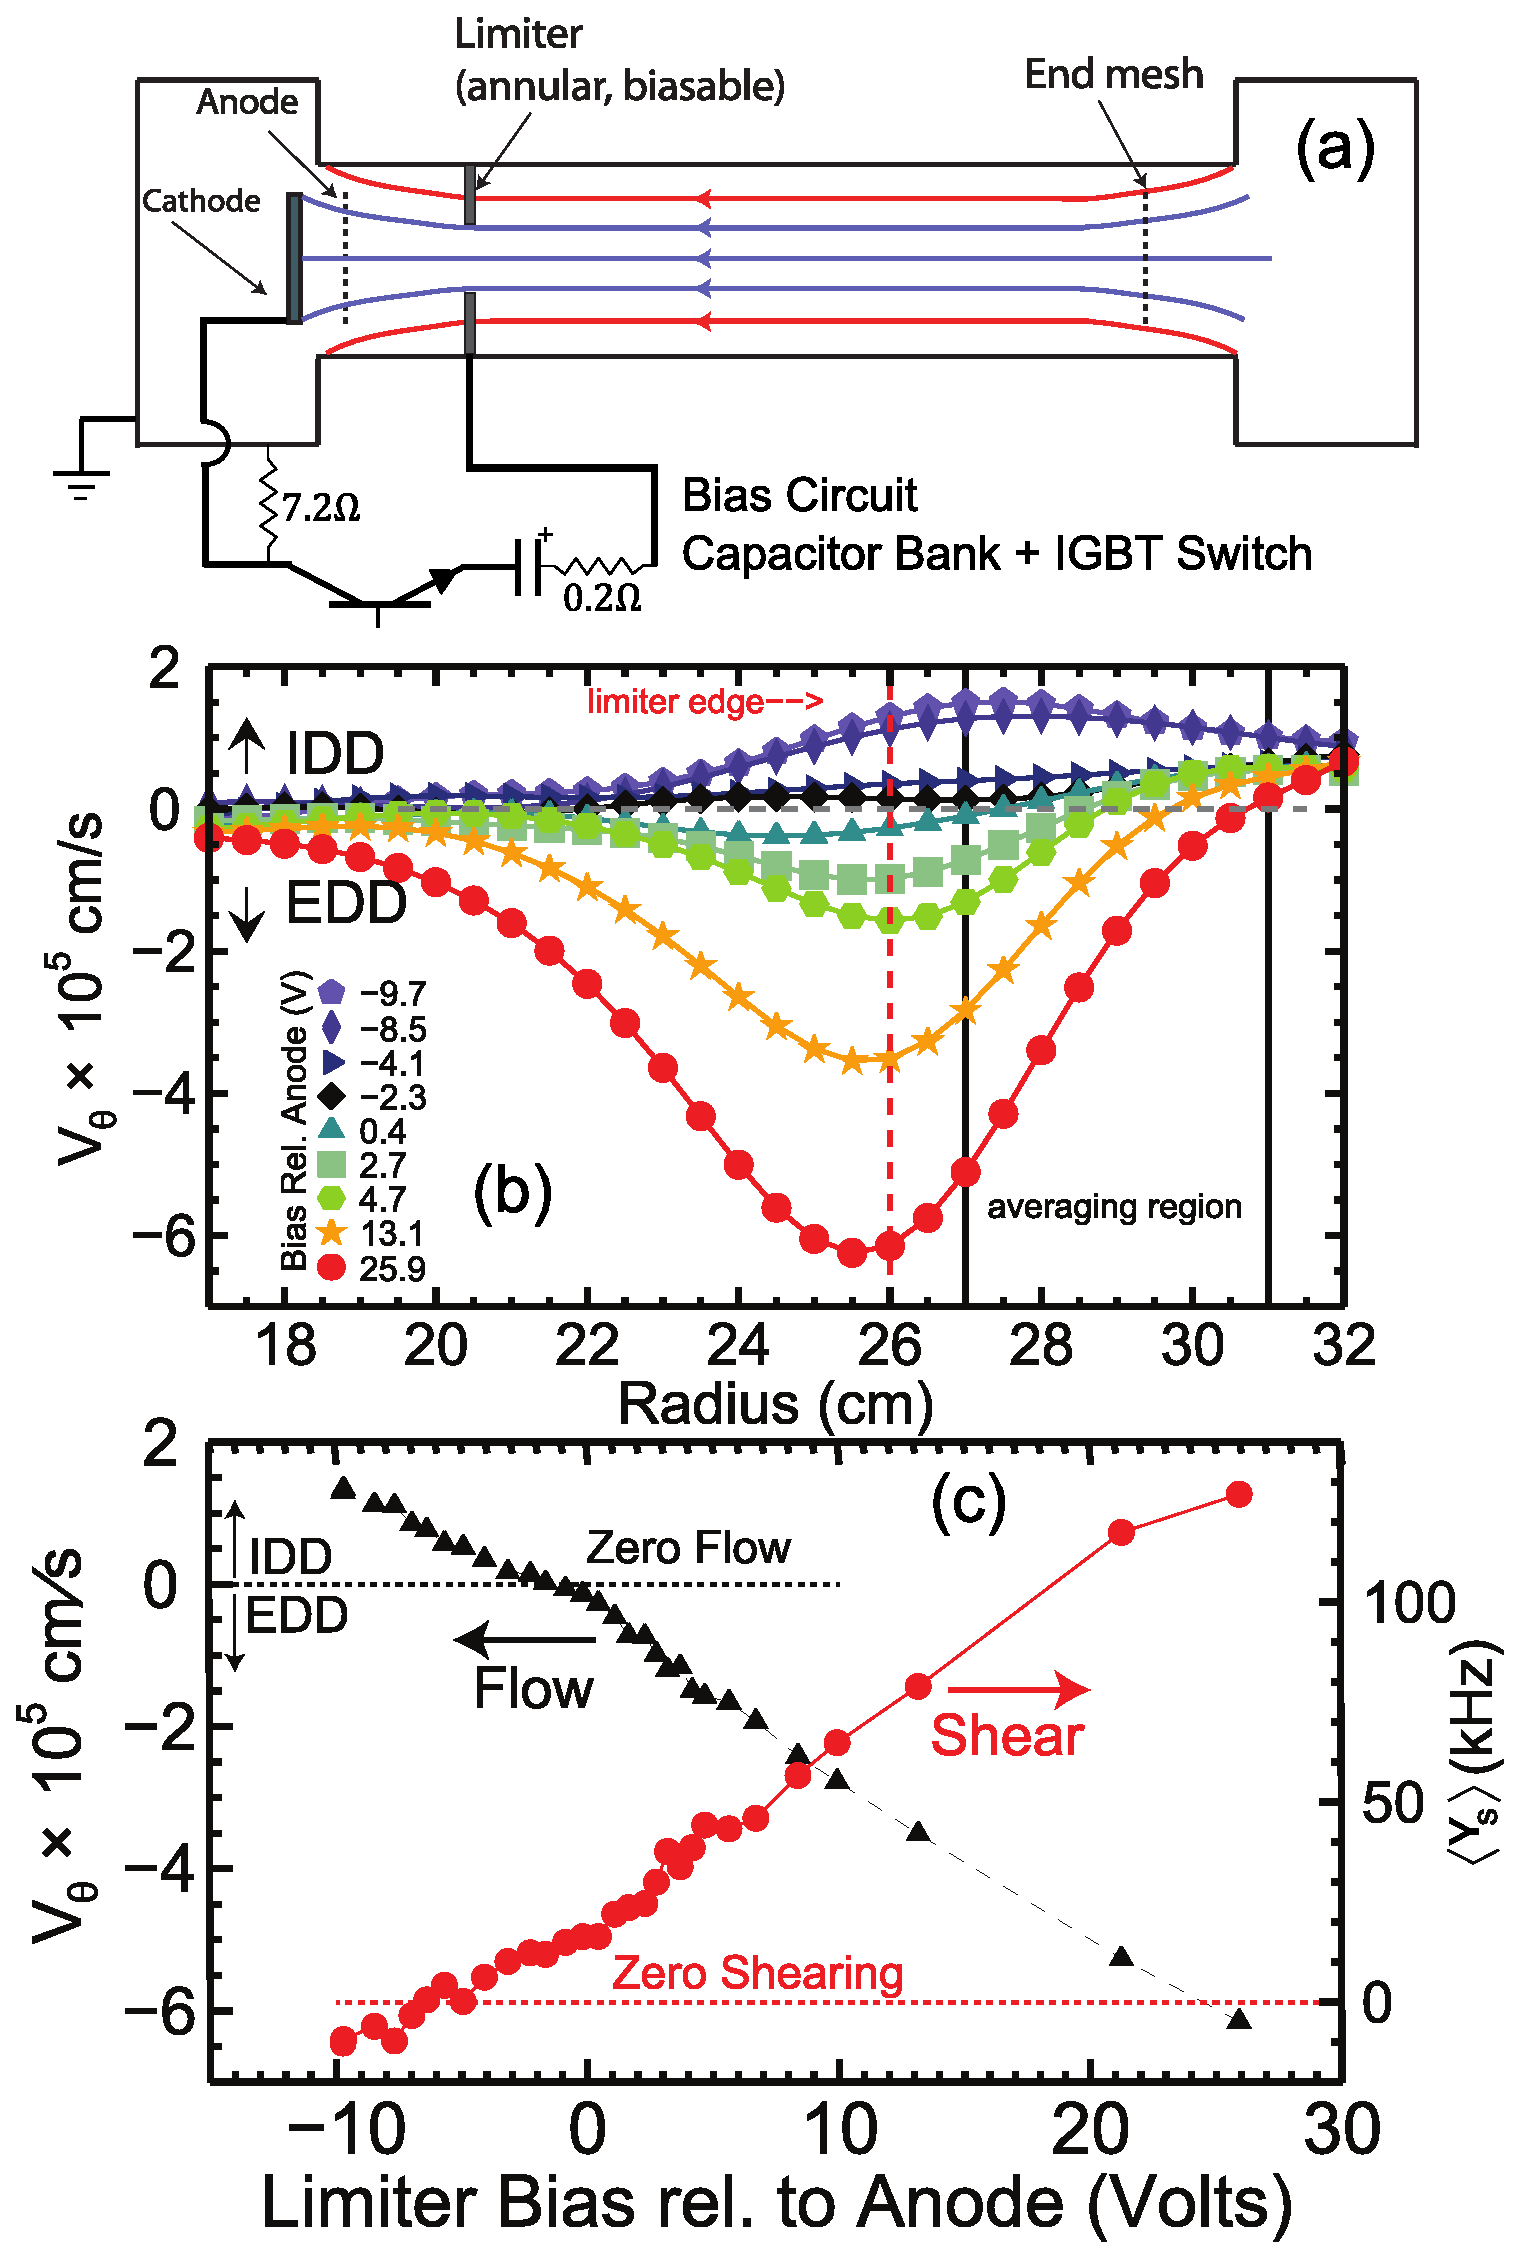
\includegraphics[width=8.5cm]{figure1.eps}}
\caption{\label{fig:velocity_flowshear} (a) Diagram of the LAPD device showing annular limiter.  (b) Velocity profiles using plasma potential from swept measurements. (c) Flow at the limiter edge (black, triangles) and mean shearing rate, averaged over $27 < r < 31$cm (red, circles).}
\end{figure}

A recent experiment on the LAPD ~\cite{schaffner12} demonstrated the ability to achieve fine and continuous control of steady-state azimuthal flow and flow shear through the use of biasable limiters. The spontaneous flow in the ion diamagnetic drift direction was first nullified and then reversed into the electron diamagnetic drift direction as bias was increased. This resulted in a continuous scan of flow shear states up to a shearing rate, $\gamma_s$, of about five times the turbulent inverse autocorrelation time  $\tau_{ac}^-1$ as measured in the unsheared state. Measurements of radial particle flux, density profiles and fluctuation amplitude showed suppression of all three quantities as a function of normalized sheared flow. Figure ??? shows the experimental results for measurements of density fluctuation amplitude, ExB or radial velocity amplitude, crossphase, particle flux, radial correlation length, and diffusivity as a function of normalized shearing rate. The shearing rates achieved span two regimes: a weak-shear regime where $\gamma_{s}\tau_{ac} < 1$ and a strong-shear regime where $\gamma_{s}\tau_{ac} > 1$.

Measurements of the steady-state correlation length were also taken for a scan of biases using a two-probe correlation plane technique. A reference probe collecting $I_{\rmdefault sat}$ is located at an axial position at the far end of the machine and placed at a single radial position. A second $I_{\rmdefault sat}$ collecting probe situated at an axial point closer to the cathode at is scanned in a rectangular grid around the projected reference point. The axial variation of the fluctuations is assumed to be low as the turbulent structures are filamentary in nature. The cross-correlation function of these two saturated current time-series is calculated for a delay time $\tau$ as
%
\begin{equation}
C(x,y,\tau) = \langle I_{ref}(x,y,t)I_{mot}(x,y,t+\tau)\rangle.
\label{eq:time_correlation}
\end{equation}
%
At $\tau = 0$, the function $C(x,y)$ shows the radial and axial extend of the fluctuation correlations giving a quantitative scale to the turbulence---that is, the smaller the correlation length, the more the plasma turbulence tends to decorrelate the fluctuations as shown in the inset of Fig.~\ref{fig:radcorr}(a) which shows the normalized correlation function $C(x,y)/C_{max}$ for an unbiased state, a minimum shear state, and a high bias state with a reference point located at 29.5cm, right in the middle of the shear layer. The black curve represents the contour line where $C(x,y)/C_{max} = 0.5$. Thus, the radial correlation length, $\Delta r_{c}$ is defined as the width of the black curve that goes through the reference point. This value is plotted in Fig.~\ref{fig:radcorr} as a function of shearing rate for various bias states, normalized to the maximum radial correlation calculated for all biases.

Finally, some parameter regimes for the shearing and density gradient length scales are presented in Fig.~\ref{LgammaL}. The shearing scale length is calculated as in $L_{\gamma} = |\nabla \ln(v_{E\times B}|^{-1}.$ This value is compared to the density gradient scale length, $L_{n} = |\nabla \ln{n}|^{-1}$ for each bias and mapped to a normalized shearing value. This plot shows that for the all of the strong shearing regime, and nearly half of the weak shearing regime, $L_{n} > L_{\gamma}$. The reverse is true only for the weakest shearing points. This quantity $L_{\gamma}/L_{n}$ can be utilized in asymptotic limits similar to the $\gamma_{s}/\tau_{ac}^{-1}$ ratio for models~\cite{leconte06}.

\section{Experimental Scaling}

\begin{figure}[!htbp]
\centerline{
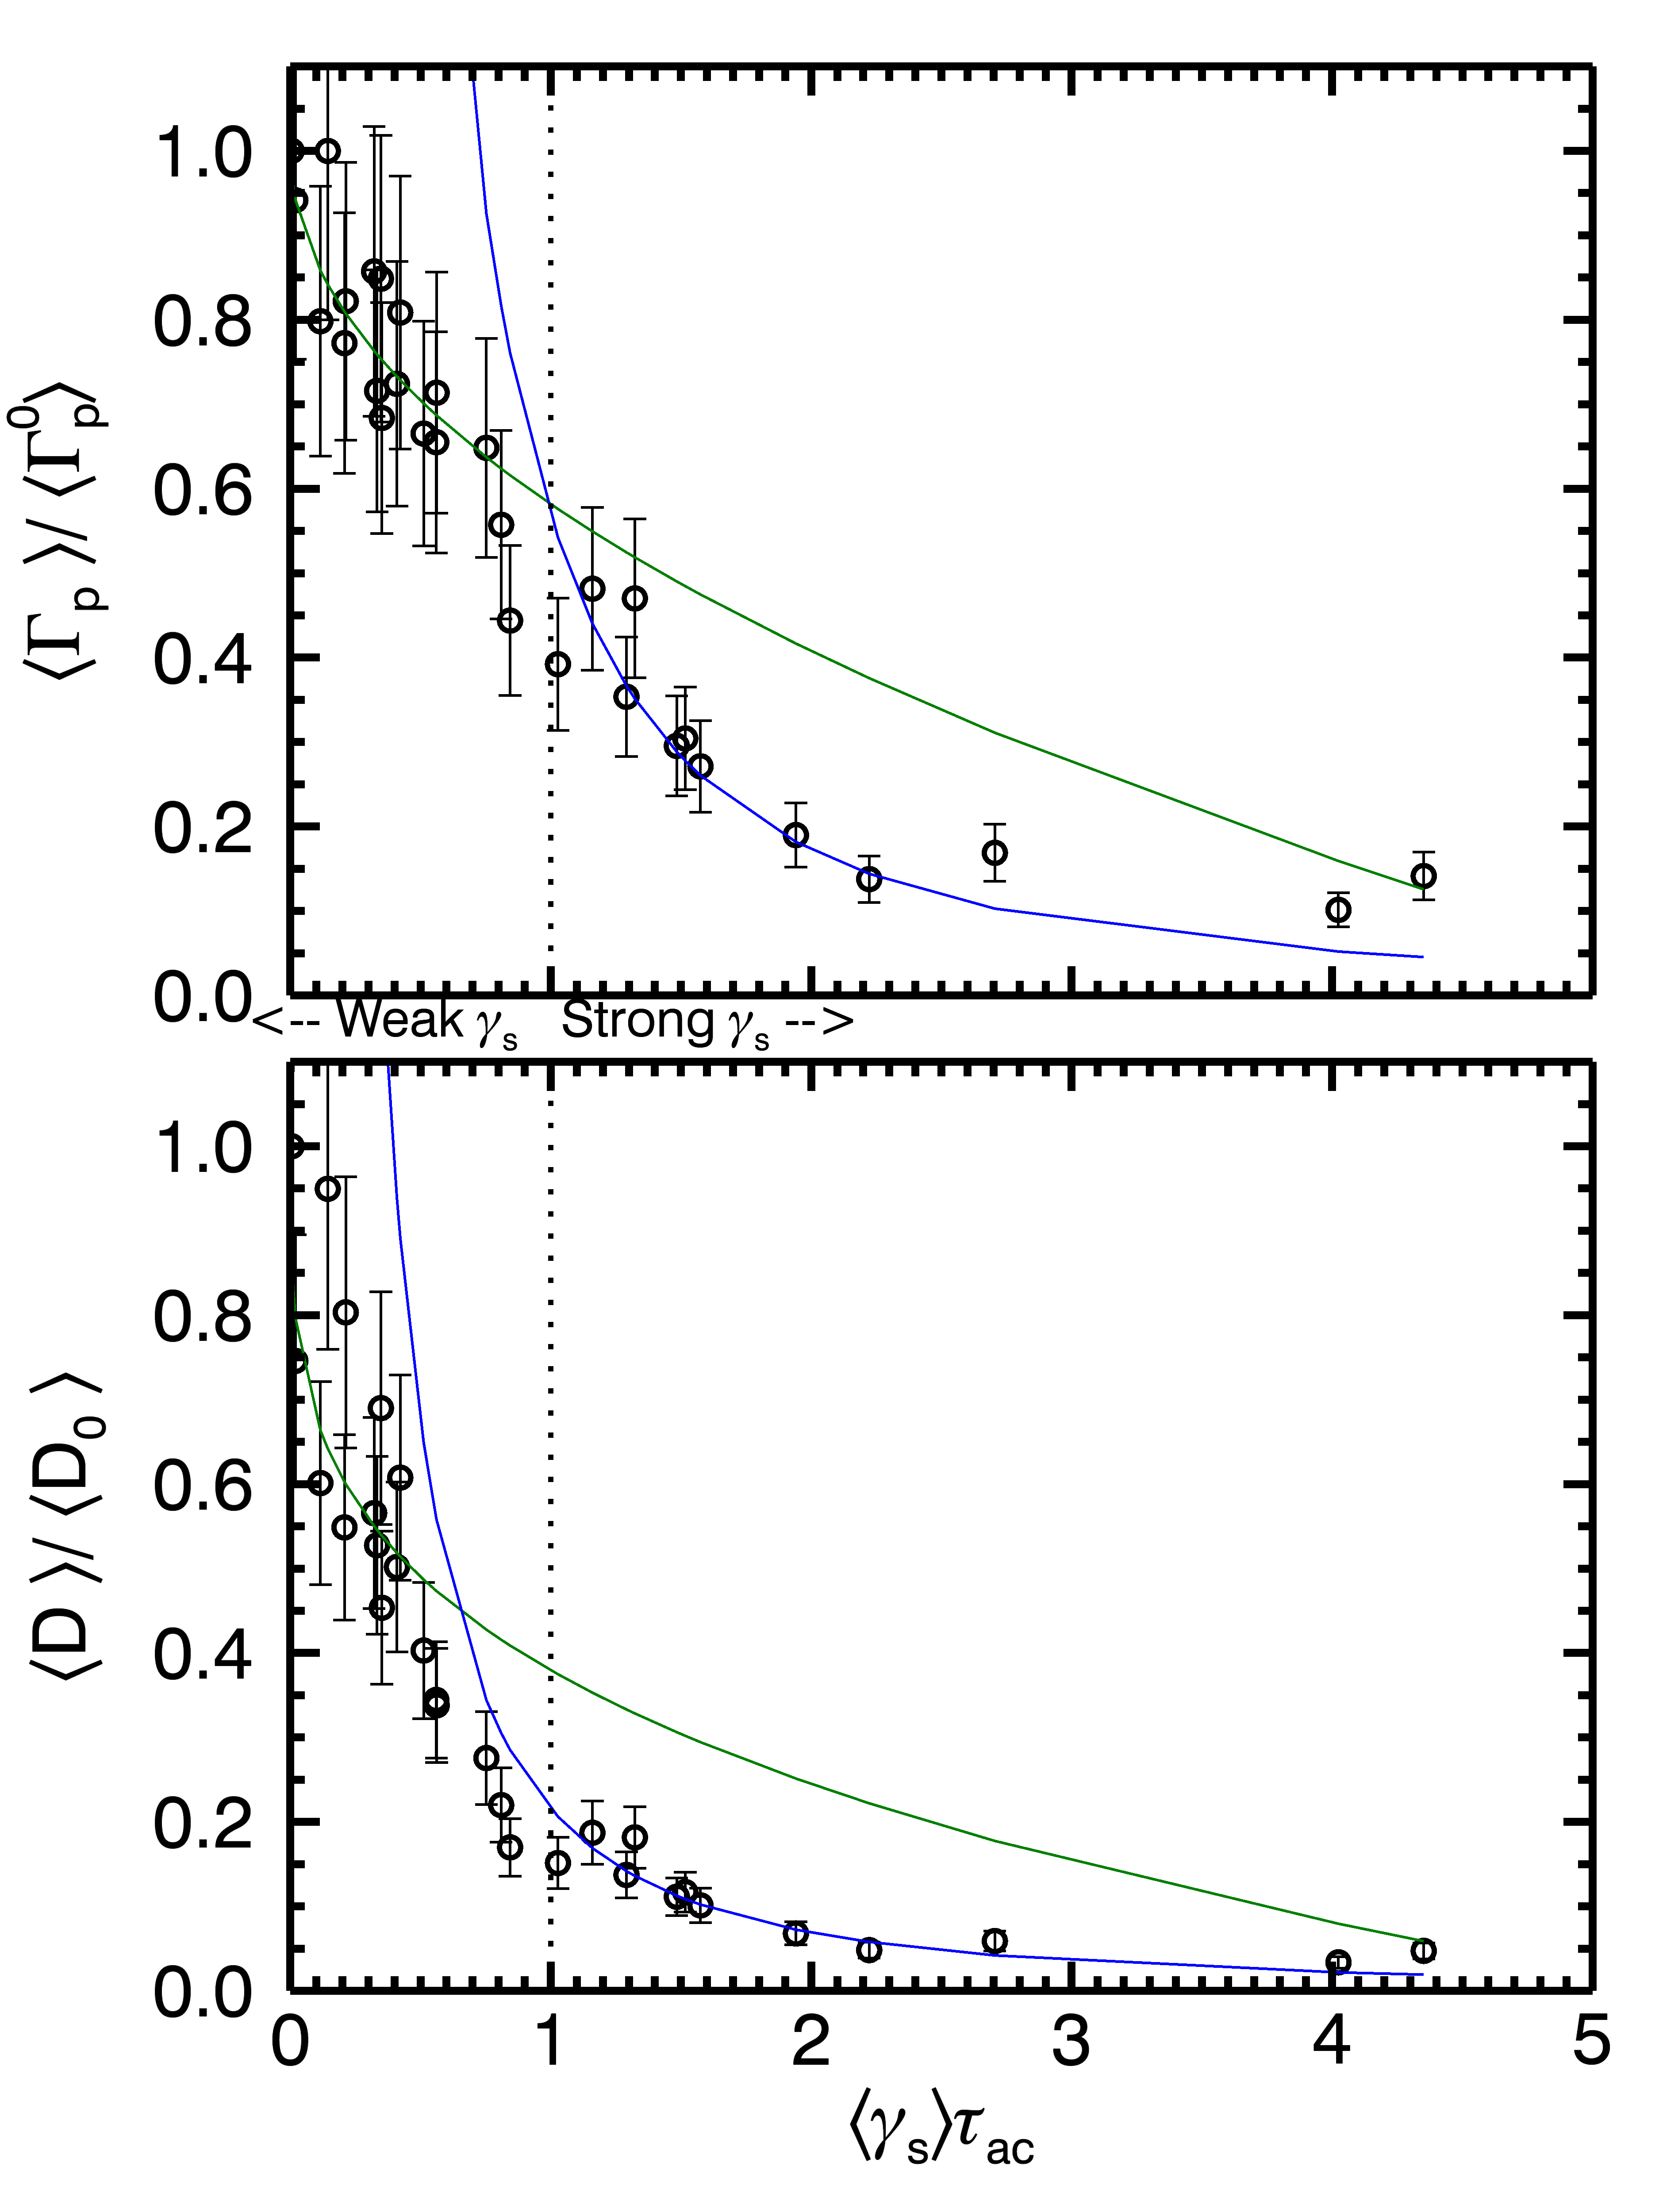
\includegraphics[width=8.5cm]{fluxandD}}
\caption{\label{fig:fluxandD} Scaling of (a)radial particle flux and (b)diffusion coefficient each normalized to the value at minimum shear, $\Gamma_{p}^{0} = 1.7\times10^{16} cm^{-2}$ and $D_{0} = 36.7 m^{2}/s$. The green curves correspond to $1-\gamma_{s}^{\nu}$ fits of the weak shear regime with $\nu = 0.501$ for flux and $\nu = 0.418$ for D. The blue curves correspond to $\gamma_{s}^{\nu}$ fits with $\nu = -1.719$ for flux and $\nu = -1.646$ for D.}
\end{figure}

\begin{figure}[!htbp]
\centerline{
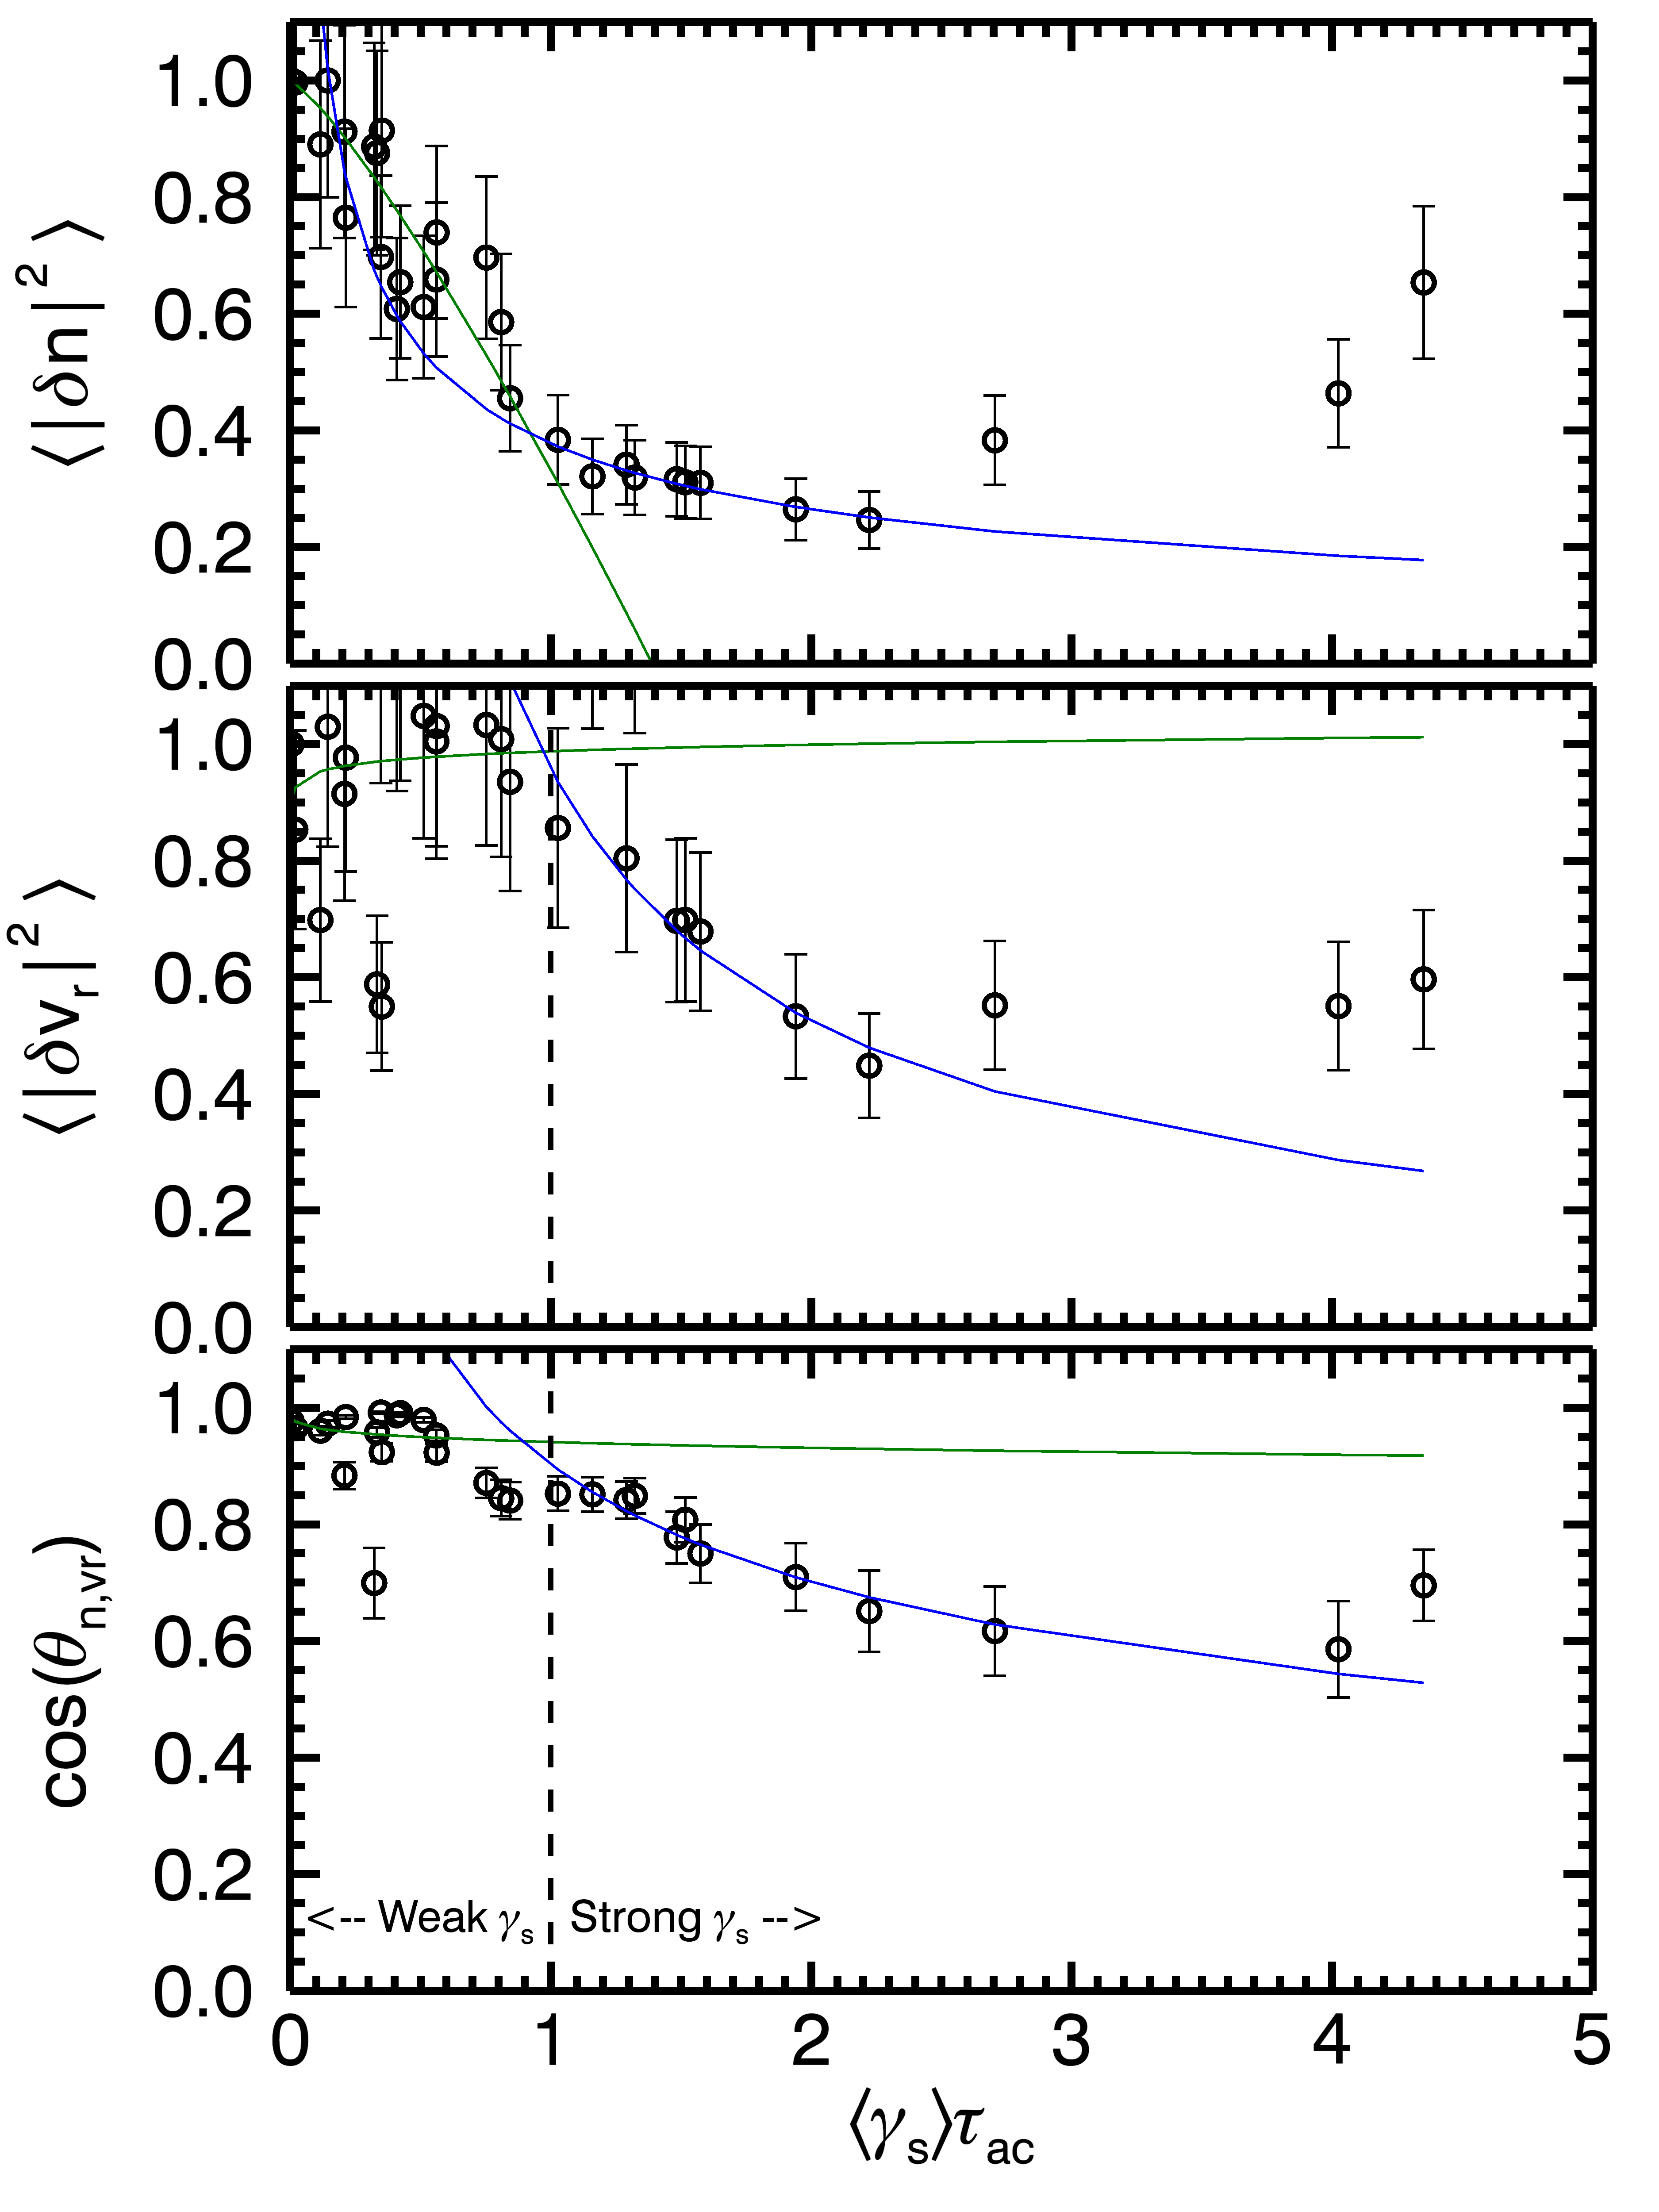
\includegraphics[width=8.5cm]{densvrcp}}
\caption{\label{fig:densvrcp} Scaling of (a)density fluctuation amplitude, (b)radial velocity fluctuation amplitude, and (c)relative crossphase between denisty and radial velocity fluctuations. Density and velocity fluctuation are each normalized to the value at minimum shear. The green curves correspond to $1-\gamma_{s}^{\nu}$ fits of the weak shear regime with $\nu = 0.501$ for flux and $\nu = 0.418$ for D. The blue curves correspond to $\gamma_{s}^{\nu}$ fits with $\nu = -1.719$ for flux and $\nu = -1.646$ for D.}
\end{figure}

\begin{figure}[!htbp]
\centerline{
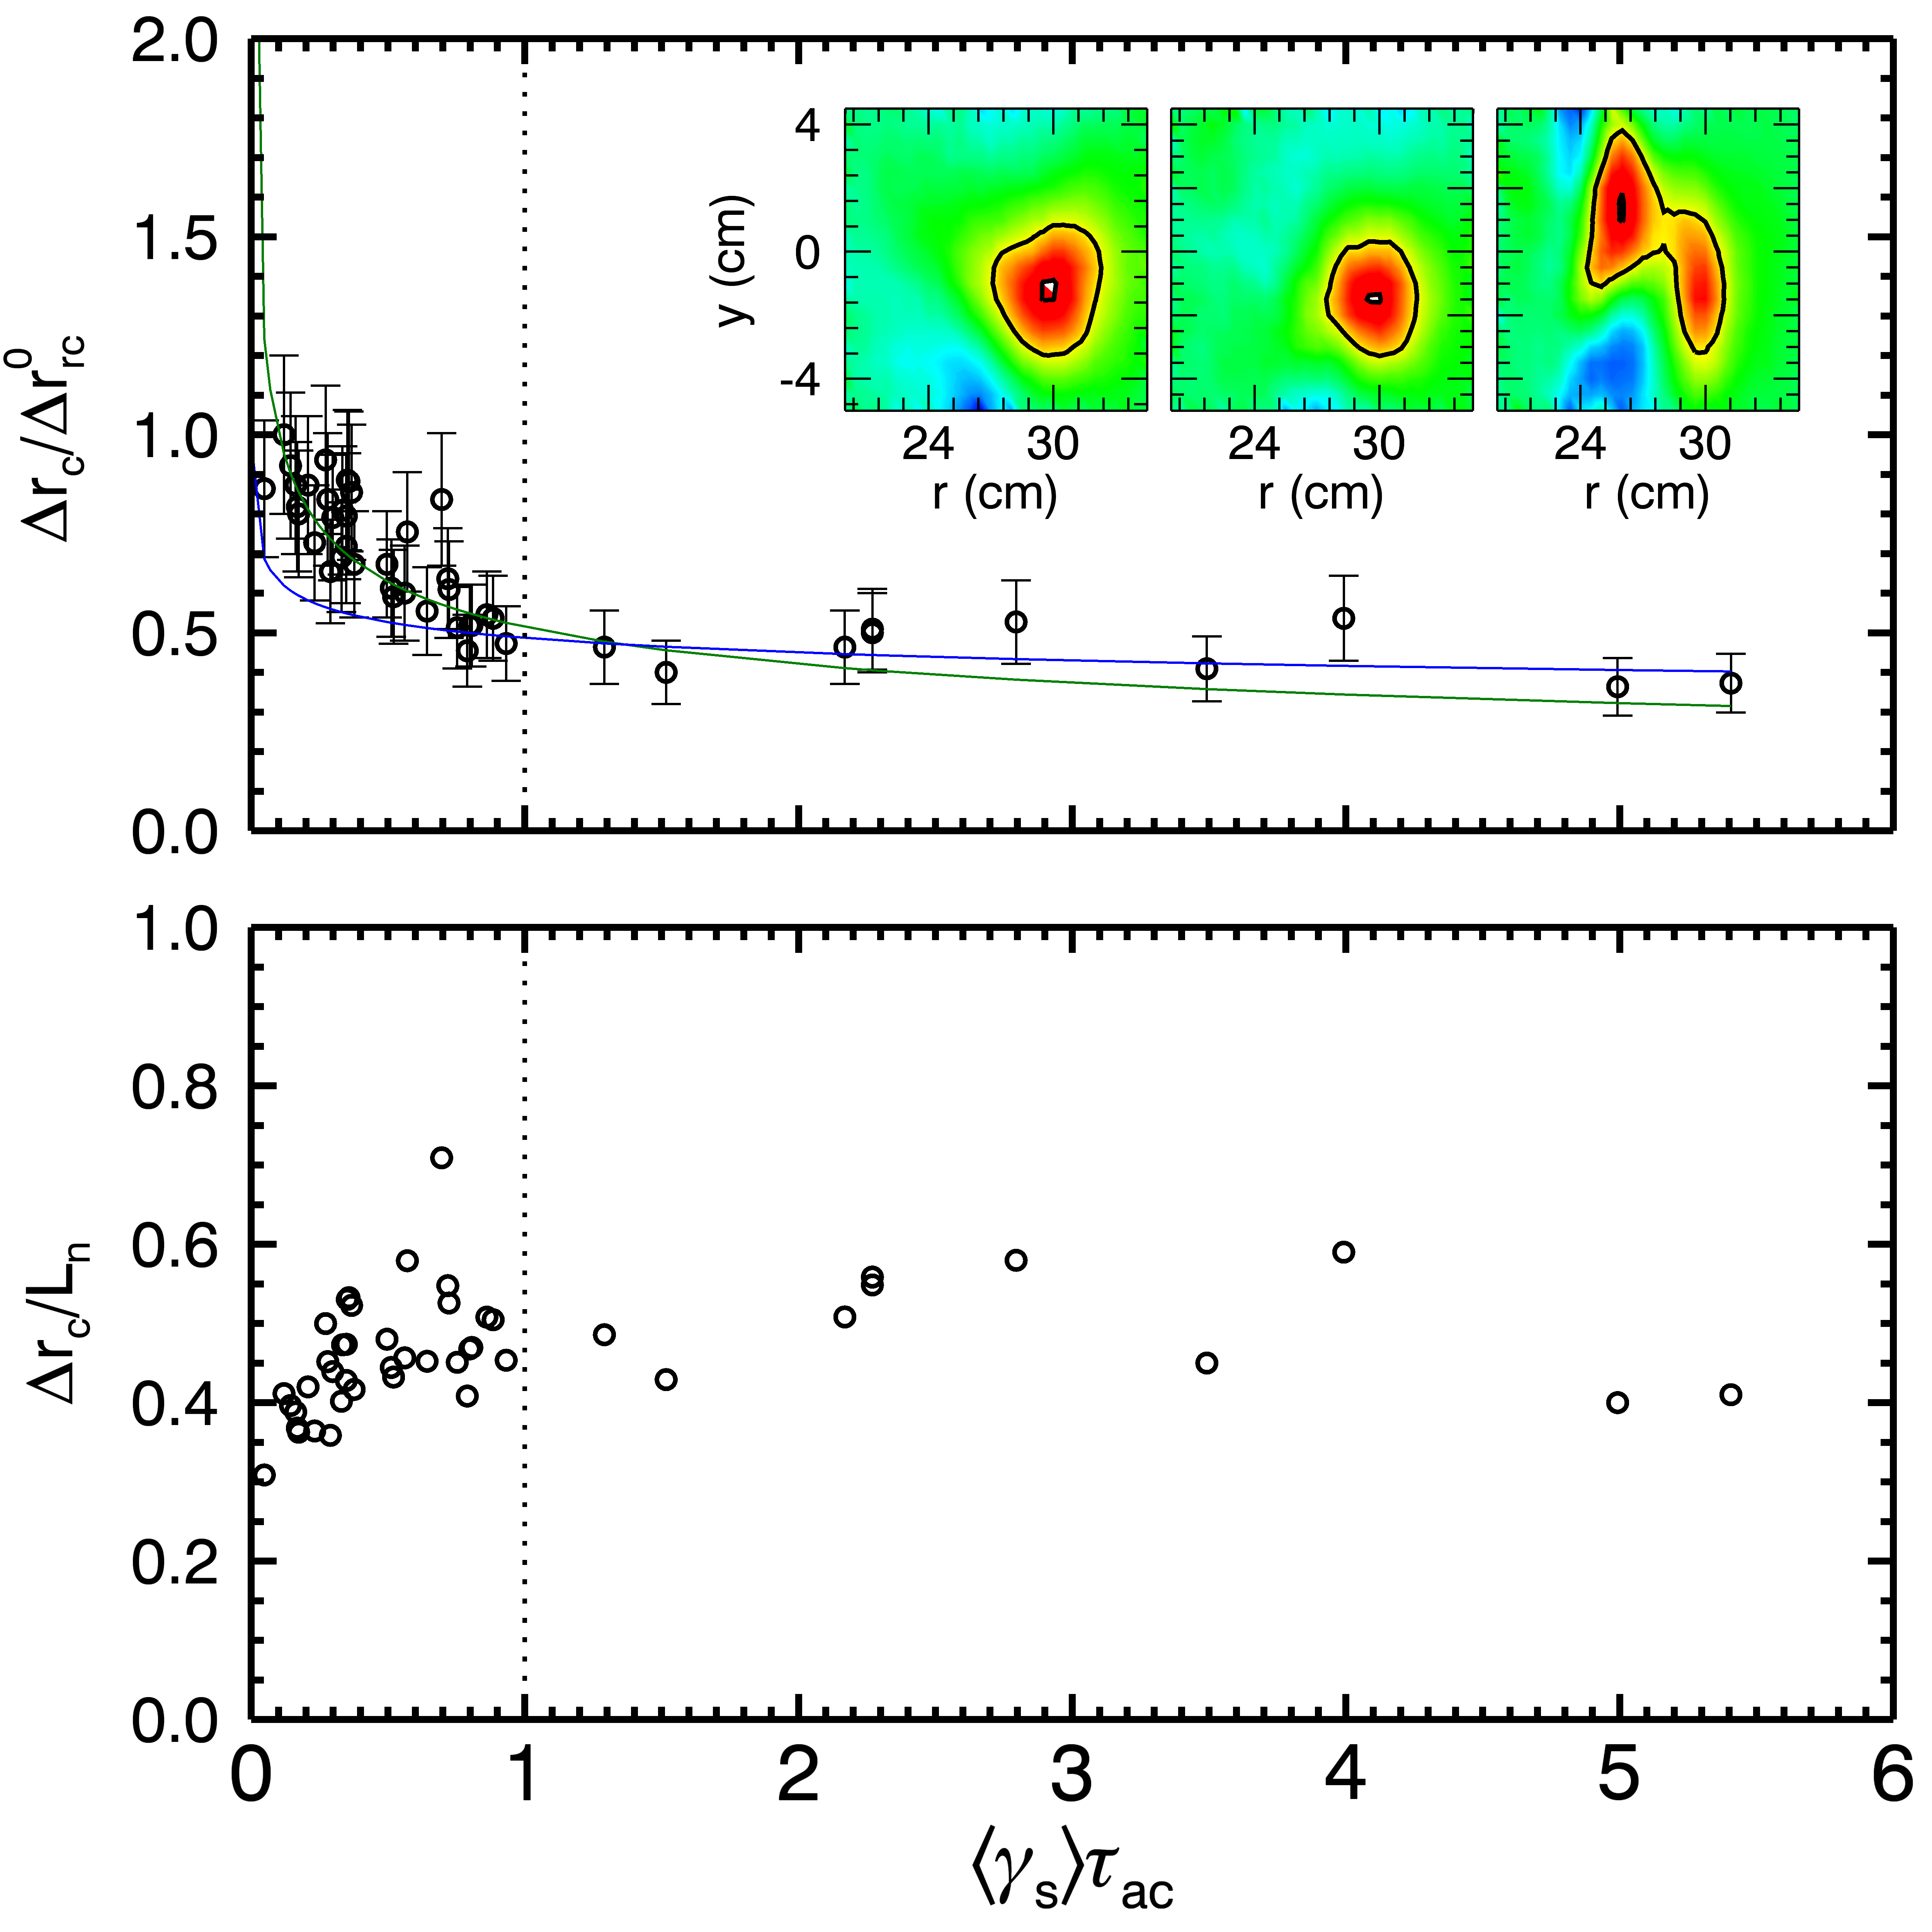
\includegraphics[width=8.5cm]{RadCorrLn}}
\caption{\label{fig:radcorr} (a)Radial correlation length normalized to maximum correlation length versus normalized shearing rate with correlation planes of unbiased, zero shear, and high bias states in the inset. (b)Ratio of radial correlation length to density gradient scale length.}
\end{figure}

\begin{figure}[!htbp]
\centerline{
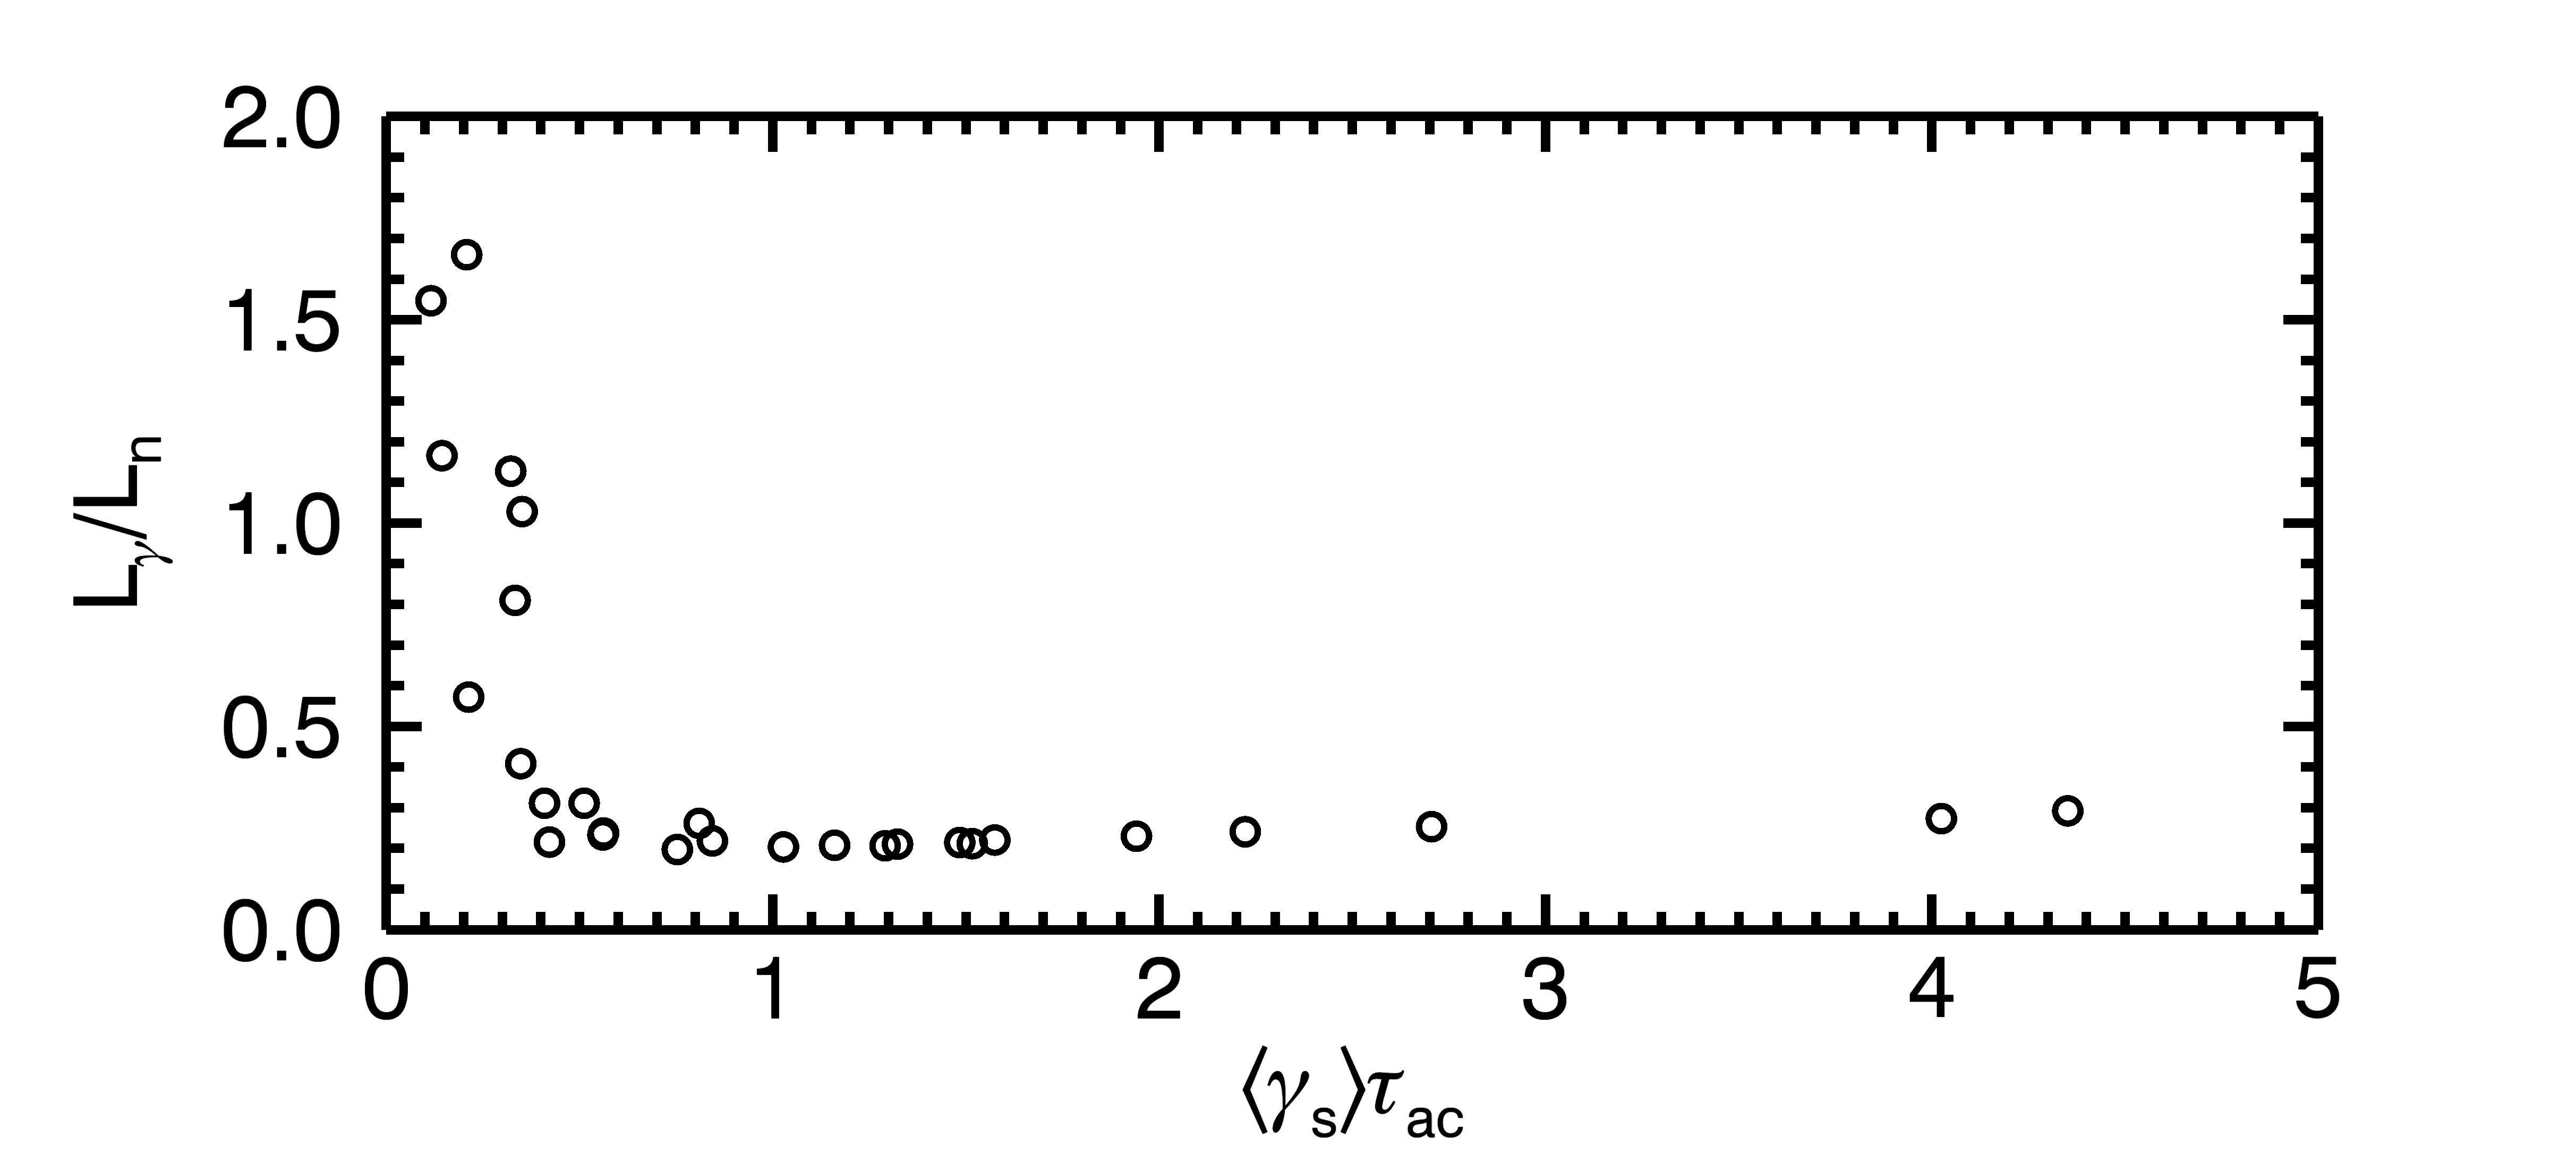
\includegraphics[width=8.5cm]{LgammaLn}}
\caption{\label{fig:LgammaLn} Ratio of shearing length scale to density gradient length scale versus normalized shearing in the radial region of 27 to 31cm.}
\end{figure}

\begin{figure}[!htbp]
\centerline{
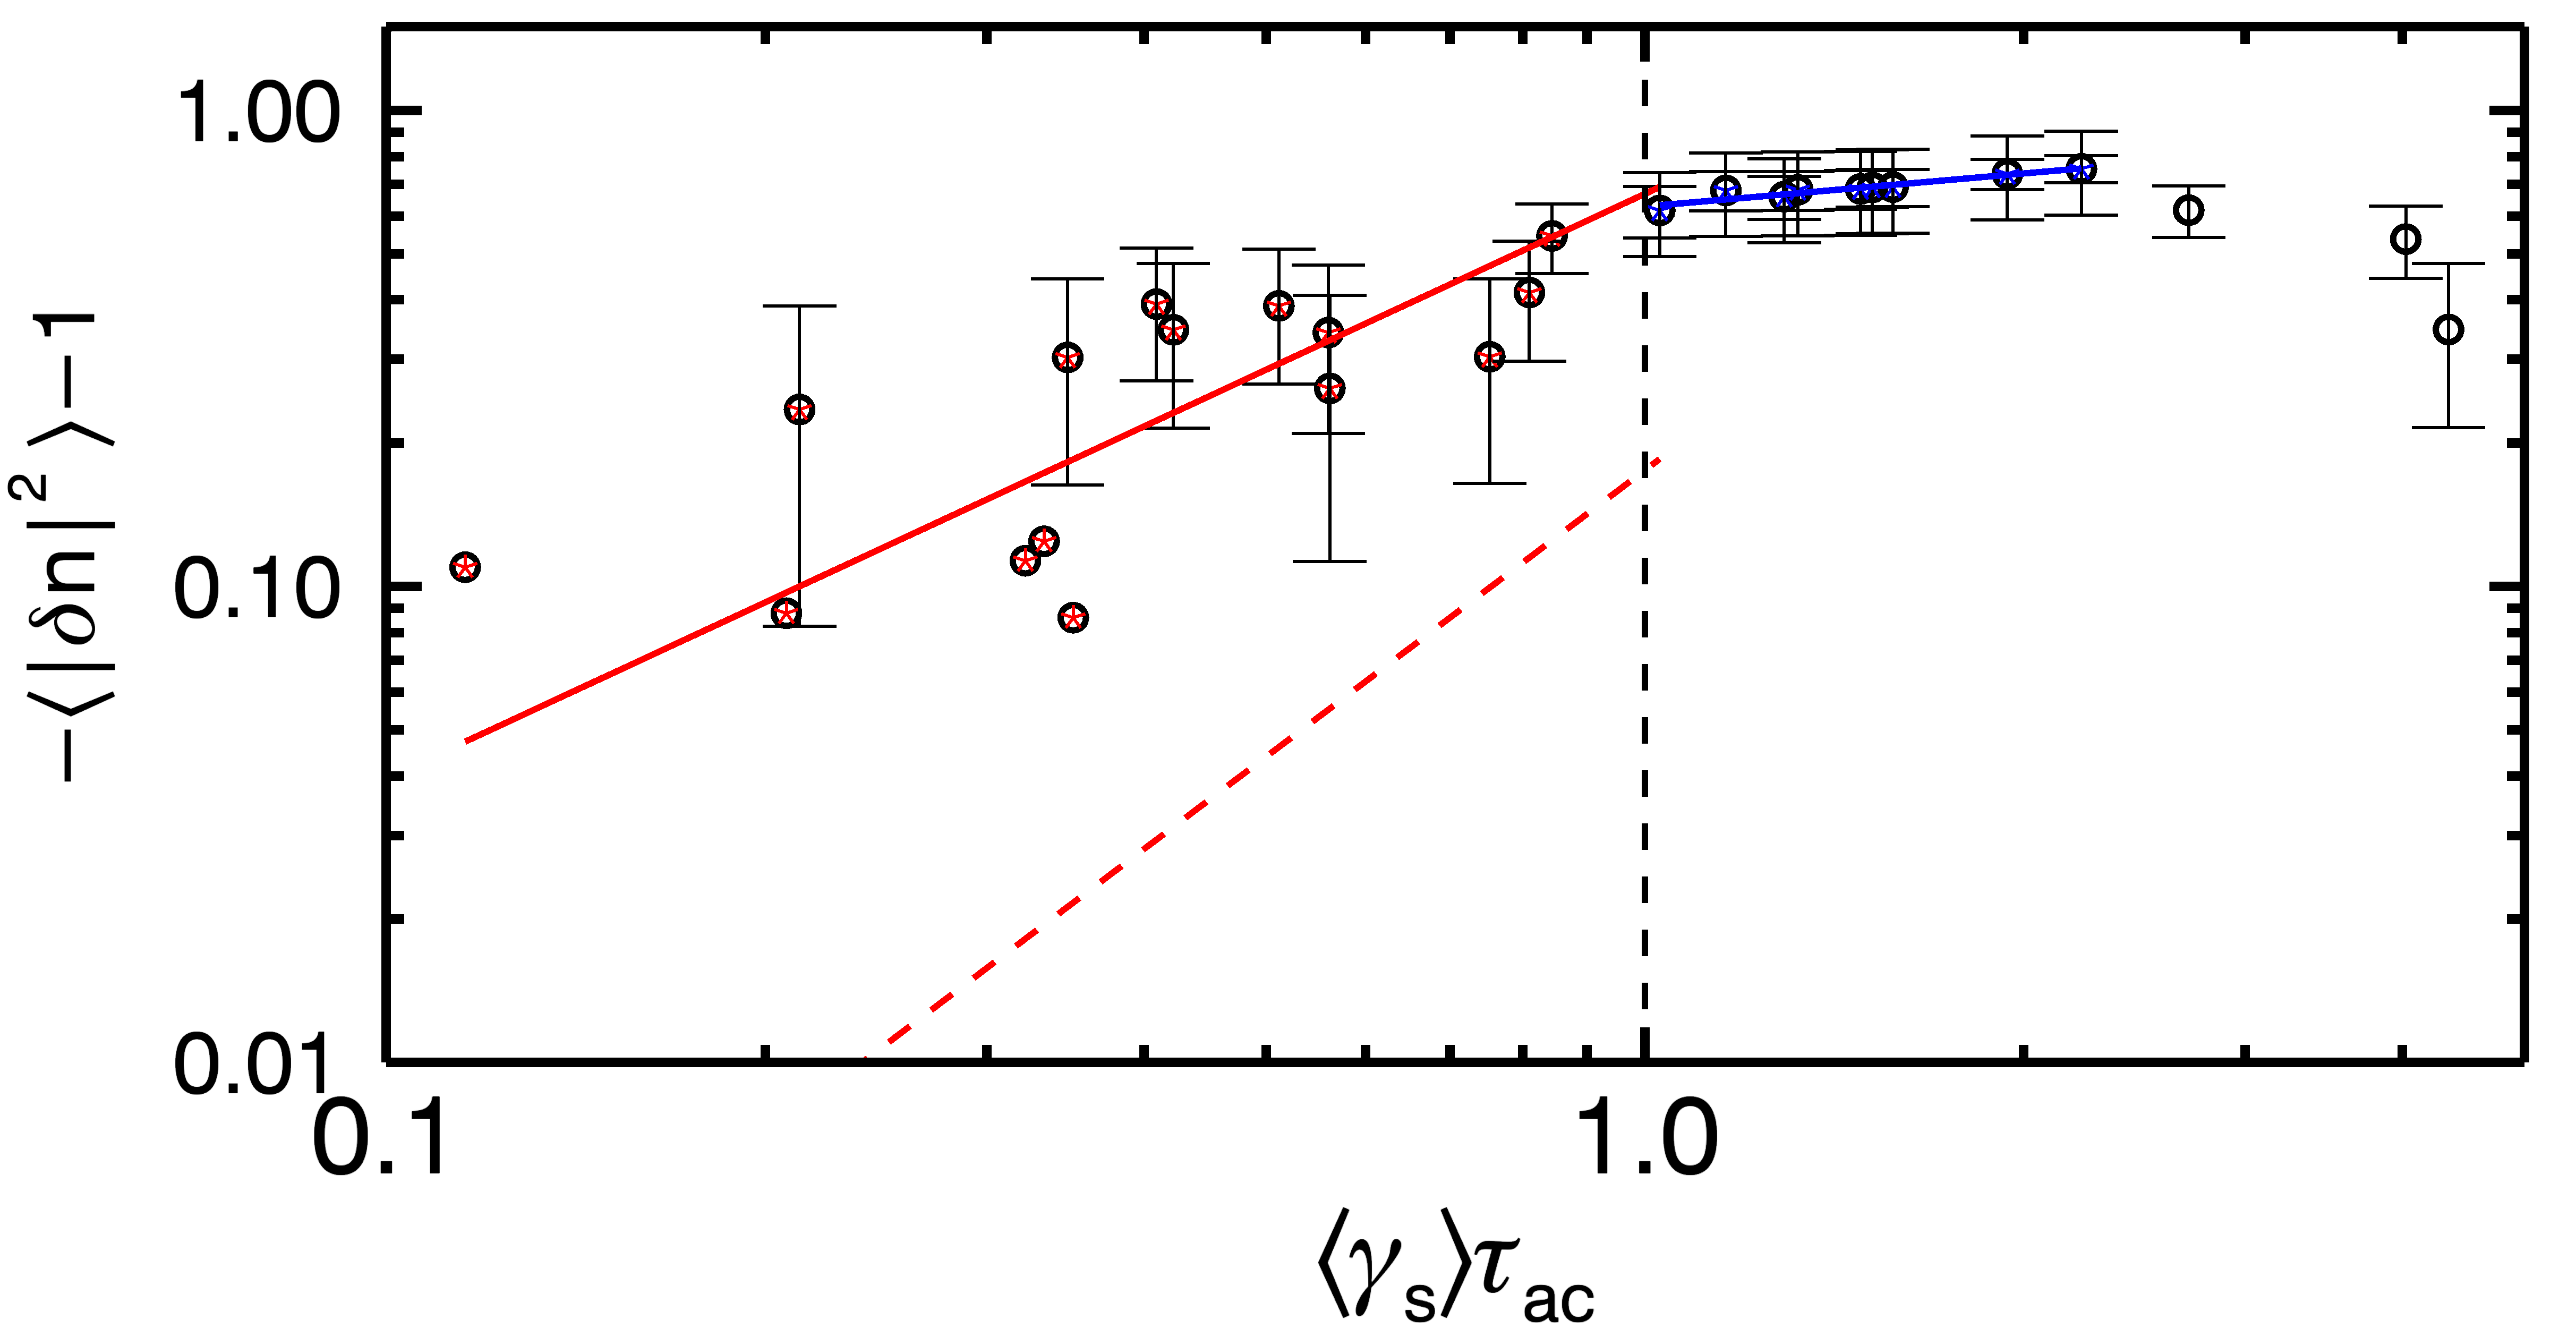
\includegraphics[width=8.5cm]{densloglog_weak}}
\caption{\label{fig:densloglog_weak} Log-Log plot of -(density fluctuation amplitude)-1 versus shearing with fit function for weak shear in solid red, Shaing scaling of 2 indicated by dashed red line. Blue line is fit for strong shearing}
\end{figure}

\begin{figure}[!htbp]
\centerline{
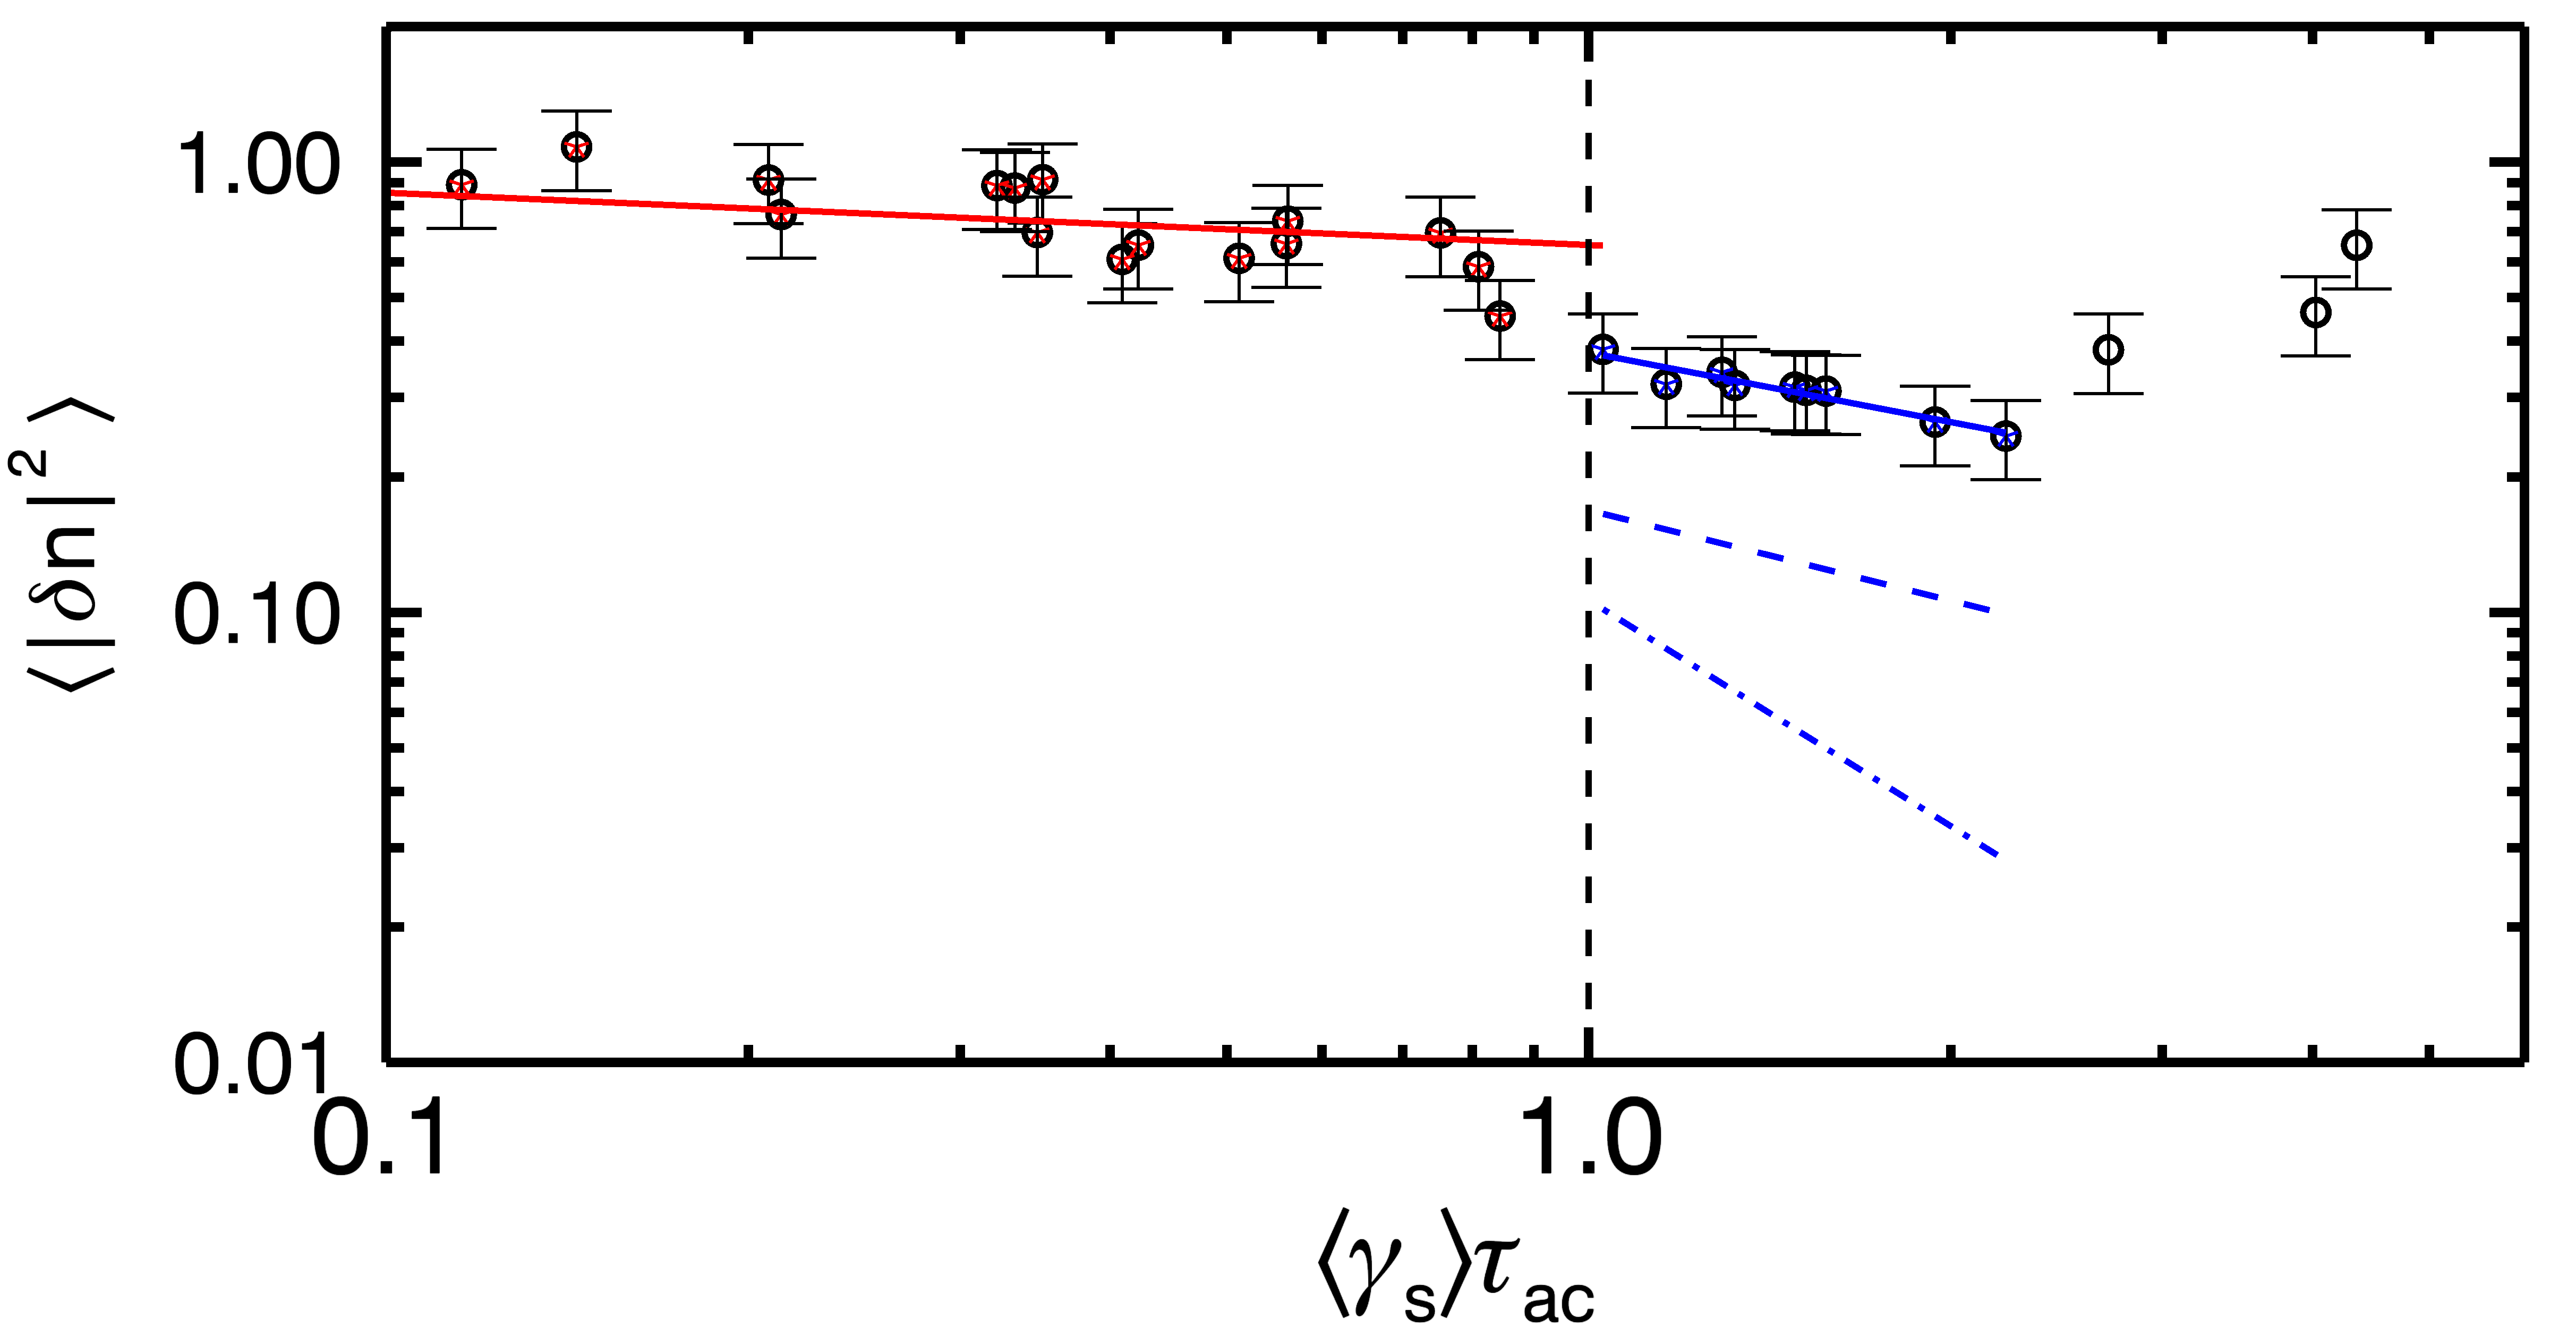
\includegraphics[width=8.5cm]{densloglog_strong}}
\caption{\label{fig:densloglog_strong} Log-Log plot of density fluctuation amplitude versus shearing with fit function for strong shear in solid blue, BDT scaling of -2/3 indicated by dashed blue line and Kim and Diamond scaling of -5/3 indicated by steeper dashed-dotted line.}
\end{figure}

\begin{table}
\caption{\label{tab:table1}Power-law fits for $|\tilde{n}^{2}|$ scaling with shear for frequencies in 350Hz to 100kHz. Model form refers to how the shearing relates to the quantity in question, with C a constant and $\nu$ the power exponent.}
\begin{ruledtabular}
\begin{tabular}{llccc}
%One&Two&\mbox{Three}&\mbox{Four}&\mbox{Five}\\
Model form&$\gamma_{s}$ regime&$\nu$&$\chi^2$&$\chi^2/ndf$\\
\hline
$\sim 1-C\gamma_{s}^\nu$&$\gamma_{s}\tau_{ac}<1$&1.228&1.091&0.0642\\
$\sim C\gamma_{s}^\nu$&$\gamma_{s}\tau_{ac}<1$&-0.116&0.1791&0.0094\\
$\sim C\gamma_{s}^\nu$&$\gamma_{s}\tau_{ac}>1$&-0.512&0.0024&0.0003\\
\end{tabular}
\end{ruledtabular}
\end{table}

\begin{table}
\caption{\label{tab:table2}Power-law fits for $|\tilde{v}_{r}^{2}|$ scaling with shear for frequencies in 350Hz to 100kHz. Model form refers to how the shearing relates to the quantity in question, with C a constant and $\nu$ the power exponent.}
\begin{ruledtabular}
\begin{tabular}{llccc}
%One&Two&\mbox{Three}&\mbox{Four}&\mbox{Five}\\
Model form&$\gamma_{s}$ regime&$\nu$&$\chi^2$&$\chi^2/ndf$\\
\hline
$\sim C\gamma_{s}^\nu$&$\gamma_{s}\tau_{ac}<1$&0.016&0.2121&0.0117\\
$\sim C\gamma_{s}^\nu$&$\gamma_{s}\tau_{ac}>1$&-0.866&0.0037&0.0005\\
\end{tabular}
\end{ruledtabular}
\end{table}

\begin{table}
\caption{\label{tab:table3}Power-law fits for $\Gamma_{p}$ scaling with shear for frequencies in 350Hz to 100kHz. Model form refers to how the shearing relates to the quantity in question, with C a constant and $\nu$ the power exponent.}
\begin{ruledtabular}
\begin{tabular}{llccc}
%One&Two&\mbox{Three}&\mbox{Four}&\mbox{Five}\\
Model form&$\gamma_{s}$ regime&$\nu$&$\chi^2$&$\chi^2/ndf$\\
\hline
$\sim 1-C\gamma_{s}^\nu$&$\gamma_{s}\tau_{ac}<1$ &0.501   &0.332    &0.0189\\
$\sim C\gamma_{s}^\nu$&$\gamma_{s}\tau_{ac}<1$   &-0.111  &0.146    &0.0077\\
$\sim C\gamma_{s}^\nu$&$\gamma_{s}\tau_{ac}>1$   &-1.719  &62.49    &5.2000\\
\end{tabular}
\end{ruledtabular}
\end{table}

\begin{table}
\caption{\label{tab:table4}Power-law fits for $cos(\theta_{nv_{r}})$ scaling with shear for frequencies in 350Hz to 100kHz. Model form refers to how the shearing relates to the quantity in question, with C a constant and $\nu$ the power exponent.}
\begin{ruledtabular}
\begin{tabular}{llccc}
%One&Two&\mbox{Three}&\mbox{Four}&\mbox{Five}\\
Model form&$\gamma_{s}$ regime&$\nu$&$\chi^2$&$\chi^2/ndf$\\
\hline
$\sim 1-C\gamma_{s}^\nu$&$\gamma_{s}\tau_{ac}<1$ &0.226   &6.1140    &0.3320\\
$\sim C\gamma_{s}^\nu$&$\gamma_{s}\tau_{ac}<1$   &-0.020  &0.0369    &0.0019\\
$\sim C\gamma_{s}^\nu$&$\gamma_{s}\tau_{ac}>1$   &-0.365  &0.0023    &0.0003\\
\end{tabular}
\end{ruledtabular}
\end{table}

\begin{table}
\caption{\label{tab:table5}Power-law fits for $D = \Gamma_{p}/\nabla{n}$ scaling with shear for frequencies in 350Hz to 100kHz. Model form refers to how the shearing relates to the quantity in question, with C a constant and $\nu$ the power exponent.}
\begin{ruledtabular}
\begin{tabular}{llccc}
%One&Two&\mbox{Three}&\mbox{Four}&\mbox{Five}\\
Model form&$\gamma_{s}$ regime&$\nu$&$\chi^2$&$\chi^2/ndf$\\
\hline
$\sim 1-C\gamma_{s}^\nu$&$\gamma_{s}\tau_{ac}<1$ &0.418   &1.4710    &0.0817\\
$\sim C\gamma_{s}^\nu$&$\gamma_{s}\tau_{ac}<1$   &-0.217  &0.4200    &0.0221\\
$\sim C\gamma_{s}^\nu$&$\gamma_{s}\tau_{ac}>1$   &-1.646  &0.0187    &0.0021\\
\end{tabular}
\end{ruledtabular}
\end{table}

\begin{table}
\caption{\label{tab:table6}Power-law fits for $\Delta r_{c}$ scaling with shear for frequencies in 350Hz to 100kHz. Model form refers to how the shearing relates to the quantity in question, with C a constant and $\nu$ the power exponent.}
\begin{ruledtabular}
\begin{tabular}{llccc}
%One&Two&\mbox{Three}&\mbox{Four}&\mbox{Five}\\
Model form&$\gamma_{s}$ regime&$\nu$&$\chi^2$&$\chi^2/ndf$\\
\hline
$\sim C\gamma_{s}^\nu$&$\gamma_{s}\tau_{ac}<1$ &-0.290 &5.8730 &0.1630\\
$\sim C\gamma_{s}^\nu$&$\gamma_{s}\tau_{ac}>1$ &-0.113 &3.7040 &0.3370\\
\end{tabular}
\end{ruledtabular}
\end{table}

The various experimentally measured quantities as functions of normalized shearing rate were fit to a power law in two ways reflecting in order to make comparisons to models of the form $1-\gamma_{s}^{\nu}$ and those those of $\gamma_{s}^{\nu}$. For the first model type, the measured quantity, y, was normalized to the value at zero shear, then transformed as $-(1-y)$. Then, taking the logarithm of both sides, a linear fit was made for points in the weak shear and in the strong shear separately. The resulting slope of the fit is taken as the power $\nu$. For the second type of model, no transformation of the quanitity y to $-(1-y)$ is made before the logarithm and fitting are taken. For a complete comparison to the wide range of model predictions made, fits were made for density fluctuation amplitude, radial particle flux, density-radial velocity fluctuation crossphase, radial velocity (ExB) fluctuation amplitude, radial correlation length, and experimental diffusivity ($\Gamma/\nabla n$). The best fits are summarized in Table~\ref{tab:table1}-~\ref{tab:table6} for each model type and for both weak and strong shear. The $\chi^{2}$ and $\chi^{2}/$ndf is also indicated in the tables.  Error bars of +/-20\% for each quanitity are shown on the plots and used in the fits, reflecting a statistical error from the number of shots used to average the quanity ($\sigma \sim 1/\sqrt{nshots}$). For weak shear fits, all points less than the weak shear cutoff $\gamma_{s}\tau_{ac}$<1 are used in the fit. For strong shear, all but the last three points are used. The last points appear to be most strongly modified by a coherent mode that develops in the highest shear and flow cases and is thought to be a break from the scaling observed in the strong shear regime. For quantities determined by summing of spectral components, including density and velocity fluctuations, flux and diffissivity, the frequenquency band used here was 350Hz to 100kHz.

\section{Results}

The best fits for scaling of density fluctuation amplitude is shown in Table~\ref{tab:table1}. For the weak shear, the direct scaling model has a slighty better $\chi^{2}$ then the $1-\gamma$ model. Both fits suggest a slightly weaker dependance on shearing with $\nu = 1.228 < 2$ for the $1-\gamma$ model, and $\nu = -0.116 < -2/3$ for the direct shearing model. In the strong shear regime, a best fit of $\nu = -0.512$ is not unreasonably far from predictions of $\nu = -2/3$ as made by BDT for example.

Particle flux scaling in Table~\ref{tab:table3} shows a much weaker scaling for weak shear then predicted by $1-\gamma$ models with $\nu = 0.501 < 2$. Meanwhile for strong shear, the direct scaling fit of $\nu = -1.719$ suggest stronger scaling then predicted by Kim and Diamond in the passive scalar model~\cite{kim03}, but less than that predicted by Terry~\cite{terry01} and by Kim and Diamond in the dynamic model~\cite{kim04}. Diffusivity in Table~\ref{tab:table5} shows a similar weak shear scaling for $1-\gamma$ models with $\nu = 0.418$ while for strong direct scaling a similar fit of $\nu = -1.646$ is found. Since $D=\Gamma_p/\nabla n$, this suggest that the effect of changing gradient tends to decrease the strength of scaling. Numerically, the direct scaling strong shear fit of $\nu = -1.646$ is close to the prediction made by Newton and Kim~\cite{newton11} of $\nu = -1.75$ for evolved turbulence with a finite correlation time.

Cosine of the the crossphase scaling in Table~\ref{tab:table4} again shows much weaker scaling in the weak shear regime with $\nu = 0.226 << 2$. Direct scaling fits in the strong shearing regime are more consistent with weak scaling as predicted by Kim and Diamond~\cite{kim03,kim04}, $\nu = -0.365 \sim -1/6$ compared to the strong scaling predicted by Terry~\cite{terry01}, $\nu = -0.365 << -3$.

A prediction for the scaling of radial velocity fluctuation amplitude is only made by Kim and Diamond~\cite{kim04} in the dynamically evolved case. Fits however for both weak and strong shear suggest a much weaker scaling than predicted. The weak shear fit actually shows a slight increase in fluctuation amplitude rather than a $\nu = -3$ scaling while in the strong shear regime a fit of $\nu = -0.866 << -4$ is found.

Finally, a fit to radial correlation length is made and compared to the only explicit prediction made by BDT~\cite{biglari90}. Neither the weak shear fit of $\nu = -0.290$ nor the strong shear of $\nu = -0.113$ is unreasonably far from the predicted value of $\nu = -1/3$, however, there is evidence that the steady-state radial correlation length is effected less by the shearing rate and more by the overall density gradient scale length. In Figure~\ref{fig:radcorr}(b) the radial correlation is shown scaled to an interpolated function of density gradient scale length resulting in a nearly constant value. This suggest that while shearing may indirectly be responsible for decreasing radial correlation rate through increased density confinement, scaling fits cannot be directly compared.

\section{Discussion}

While the large variation in shearing suppression scaling fits for upwards of six turbulent quantities makes very careful verification difficult, there an a number of conclusions that can be drawn from this analysis. First both analytic predictions and the experimental results from this dataset show a distinct difference in scaling between the weak and low shear regimes. Moreover, the fits in the weak shear regime generally compare more favorably to values made by the direct scaling $\gamma_{s}^{\nu}$ model form then to the $1-\gamma_{s}^{\nu}$ form as the closest fit to the frequently predicted $1-\gamma_{s}^{2}$ curve comes from the density fluctuation amplitude scaling while fits for flux, crossphase, diffusivity are all much less than 2. These results also shed some light on the mechanisms involved in the reduction of flux due to shearing showing density fluctuation amplitude reduction being a more significant contributer compared to crossphase change. The fits show a much more favorable comparison to weak crossphase scaling predictions then to strong, and while density amplitude scaling are generally weaker then predicted, they are closer to the prediction than the crossphase counterparts. Comparison of velocity fluctuation to prediction suggest that the dynamic modeling of the flow may not be as important in LAPD plasmas. Finally, as indicated by the wide range of predictions, the scaling of shear suppression may be dependent on the nature of the turbulence at hand. Many of the turbulence models are mode specific such as pressure-gradient turbulence for the Terry, Ware models or Rotational interchange for the later Kim, Diamond models. However, neither model fits the LAPD results very well which itself is likely a combination of pressure-gradient and rotational interchange turbulence. For future model development and comparison to these results, it may be worthwhile to make predictions based on specific LAPD type turbulence.

\providecommand{\noopsort}[1]{}\providecommand{\singleletter}[1]{#1}%
\begin{thebibliography}{10}

%shearing theory
\bibitem{burrell99}
K. Burrell, Phys. Plasmas {\bf 6},  4418  (1999).

\bibitem{oost03}
G. Van Oost and J. Adamek and V. Antoni and P. Balan and J.A. Boedo and P. Devynck and I. Duran and L. Eliseev and J.P. Gunn and M. Hron and C. Ionita and S. Jachmich and G.S. Kirnev and E. Martines and A. Melnikov and R. Schrittwieser and C. Silva and J. Stockel and M. Tendler and C. Varandas and M. Van Schoor and V. Vershkov and R.R. Weynants, Plas. Phys. Control Fusion {\bf 48}, 621 (2003).

\bibitem{sakai93}
O. Sakai and Y. Yasaka and R. Itatani, Phys. Rev. Lett. {\bf 70},  4071 (1993).

\bibitem{burrell97}
K. Burrell, Phys. Plasmas {\bf 4},  1499  (1997).

\bibitem{terry00}
P. Terry, Rev. Mod. Phys. {\bf 72},  109  (2000).

\bibitem{taylor89}
R.J. Taylor and M.L. Brown and B.D. Fried and H. Grote and J.R. Liberati and G.J. Morales and P. Pribyl and D. Darrow and M. Ono, Phys. Rev. Lett. {\bf 63},  2365  (1989).

\bibitem{weynants92}
R.R. Weynants and G. Van Oost and G. Bertschinger and J. Boedo and P. Brys and T. Delvigne and K.H. Dippel and F. Durodie and H. Euringer and K.H. Finken and D.S. Gray and J.D. Hey and D.L. Hillis and J.T. Hogan and L. Konan and R. Leners and A.M. Messian and A. Pospieszczyck and U. Samm and R.P. Schorn and B. Schweer and G. Telesca and R. Vannieuwenhove and P.E Vandenplas, Nucl. Fusion {\bf 32},  837  (1992).

\bibitem{weynants98}
R.R. Weynants and S. Jachmich and G. Van Oost, Plas. Phys. Control Fusion {\bf 40}, 635 (1998).

\bibitem{boedo00}
J. Boedo and D. Gray and S. Jachmich and R. Conn and G.P. Terry and G. Tynan and G. Van Oost and R.R. Weynants and TEXTOR Team, Nucl. Fusion {\bf 40},  7  (2000).

\bibitem{boedo02}
J.A. Boedo and D.S. Gray and P.W.Terry and S. Jachmich and G.R. Tynan and R.W. Conn and TEXTOR-94 Team, Nucl. Fusion, {\bf 42}, 117 (2002).

\bibitem{schaffner12}
D.A. Schaffner and T.A. Carter and G.D. Rossi and D.S. Guice and J.E. Maggs and S.Vincena and B. Friedman, Phys. Rev. Lett. {\bf 109}, 135002 (2012).

\bibitem{terry06}
P.W. Terry and R. Gatto, Phys. Plasmas {\bf 13}, 062309 (2006).

\bibitem{biglari90}
H. Biglari and P.H. Diamond and P.W. Terry, Phys. Fluids B. {\bf 2},  1  (1990).

\bibitem{shaing90}
K.C. Shaing and E.C. Crume and W.A. Houlberg, Phys. Fluids B {\bf 2}, 6 (1990).

\bibitem{zhang92}
Y.Z. Zhang and S.M. Mahajan, Phys. Fluids B {\bf 4}, 1385 (1992).

\bibitem{zhang93}
Y.Z. Zhang and S.M. Mahajan, Phys. Fluids B {\bf 5}, 7 (1993).

\bibitem{ware96}
A.S. Ware and P.W. Terry and P.H. Diamond and B.A. Carreras, Plasma Phys. Control Fusion {\bf 38},  1343  (1996).

\bibitem{ware98}
A.S. Ware and P.W. Terry and B.A. Carreras and P.H. Diamond, Phys. Plasmas {\bf 5}, 173 (1998).

\bibitem{terry01}
P.W. Terry and D.E. Newman and A.S. Ware, Phys. Rev. Lett. {\bf 87}, 185001  (2001).

\bibitem{kim03}
E.-J. Kim and P.H. Diamond, Phys. Rev. Lett. {\bf 90}, 7 (2003).

\bibitem{kim04}
E.-J. Kim and P.H. Diamond, Phys. Plasmas {\bf 11},  10  (2004).

\bibitem{leconte06}
M. Leconte and P. Beyer and S. Benkadda and X.Garbet, Phys. Plasmas {\bf 13} 112301 (2006).

\bibitem{newton07}
A.P.L. Newton and E.-J. Kim, Phys. Plasmas {\bf 14}, 122306 (2007).

\bibitem{newton11}
A.P.L. Newton and E.-J. Kim, Phys. Plasmas {\bf 18}, 052305 (2011).

\bibitem{gek91}
W. Gekelman and H. Pfister and Z. Lucky and J. Bamber and D. Leneman and J. Maggs, Rev. Sci. Instrum. {\bf 62},  2875  (1991).

%\bibitem{kim90}
%Y.B. Kim and P.H. Diamond and H. Biglari and P.W. Terry, Phys. Fluids B {\bf 2}, 9 (1990).

%\bibitem{wagner82}
%F. Wagner {\it et~al.}, Phys. Rev. Lett. {\bf 49},  1408  (1982).

%\bibitem{silva06}
%C. Silva {\it et~al.}, Plas. Phys. Control Fusion {\bf 48},  727  (2006).

%\bibitem{maggs07}
%J. Maggs {\it et~al.}, Phys. Plasmas {\bf 14},  052507  (2007).

%\bibitem{carter09}
%T. Carter and J. Maggs, Phys. Plasmas {\bf 16},  012304  (2009).

%\bibitem{tynan09}
%G. Tynan {\it et~al.}, Plasma Phys. Control Fusion {\bf 51}, 113001  (2009).

%\bibitem{amatucci96}
%W.E. Amatucci {\it et~al.}, Phys. Rev. Lett. {\bf 77},  1978  (1996).

%\bibitem{jass72}
%D. Jassby, Phys. Fluids {\bf 15},  9  (1972).

%\bibitem{holland04}
%C. Holland {\it et~al.}, Rev. Sci. Inst. {\bf 75},  10
%  (2004).

%\bibitem{zhou12}
%S. Zhou {\it et~al.}, Phys. Plasmas {\bf 19},  012116  (2012).

%\bibitem{powers74}
%E. Powers, Nucl. Fusion {\bf 14},  749  (1974).

%\bibitem{umansky11}
%M. Umansky {\it et~al.}, Phys. Plasmas {\bf 18},  055709  (2011).

%\bibitem{beall82}
%J.M. Beall and Y.C. Kim and E.J. Powers, J. Appl. Phys. {\bf 53}, 6, {1982}.

\end{thebibliography}

\end{document}
